%% --------------------------------------------------------
%% Thesis.tex -- MAIN FILE (the one that you compile with LaTeX)
%% --------------------------------------------------------

% Set up the document
\documentclass[a4paper, 11pt, twoside]{Thesis}  % Use the "Thesis" style, based on the ECS Thesis style by Steve Gunn
\graphicspath{Figures/}  % Location of the graphics files (set up for graphics to be in PDF format)

% Include any extra LaTeX packages required
%\usepackage[square, numbers, comma, sort&compress]{natbib}  % Use the "Natbib" style for the references in the Bibliography


\usepackage[english,greek]{babel}
%\usepackage{ucs}
\usepackage[utf8]{inputenc}

\usepackage{algorithm2e}
%\usepackage[T1]{fontenc}
\usepackage{listings}
\usepackage{verbatim}  % Needed for the "comment" environment to make LaTeX comments
\usepackage{vector}  % Allows "\bvec{}" and "\buvec{}" for "blackboard" style bold vectors in maths
\hypersetup{urlcolor=blue, colorlinks=true}  % Colours hyperlinks in blue, but this can be distracting if there are many links.

%% --------------------------------------------------------
\begin{document}
\frontmatter      % Begin Roman style (i, ii, iii, iv...) page numbering

% Set up the Title Page
\title  {Μελέτη και Αξιολόγηση Tεχνικών Ιδιωτικότητας στην Ανάλυση Δεδομένων}
\authors  {\texorpdfstring
            {\href{your web site or email address}{Γεράσιμος Βαρδακαστάνης}}
            {Author Name}
            }
\addresses 
{\groupname\\\deptname\\\univname}  % Do not change this here, instead these must be set in the "Thesis.cls" file, please look through it instead
\date       {\today}
\subject    {}
\keywords   {}

\maketitle
%% ----------------------------------------------------------------

\setstretch{1.3}  % It is better to have smaller font and larger line spacing than the other way round

% Define the page headers using the FancyHdr package and set up for one-sided printing

\fancyhead{}  % Clears all page headers and footers
\rhead{\thepage}  % Sets the right side header to show the page number
\lhead{}  % Clears the left side page header

\pagestyle{fancy}  % Finally, use the "fancy" page style to implement the FancyHdr headers

%% ----------------------------------------------------------------
% Declaration Page required for the Thesis, your institution may give you a different text to place here
%\Declaration{
%\addtocontents{toc}{\vspace{1em}}  % Add a gap in the Contents, for aesthetics

%I, AUTHOR NAME, declare that this thesis titled, `THESIS TITLE' and the work presented in it are my own. I confirm that:

%\begin{itemize} 
%\item[\tiny{$\blacksquare$}] This work was done wholly or mainly while in candidature for a research degree at this University.
 
%\item[\tiny{$\blacksquare$}] Where any part of this thesis has previously been submitted for a degree or any other qualification at this University or any other institution, this has been clearly stated.
 
%\item[\tiny{$\blacksquare$}] Where I have consulted the published work of others, this is always clearly attributed.
 
%\item[\tiny{$\blacksquare$}] Where I have quoted from the work of others, the source is always given. With the exception of such quotations, this thesis is entirely my own work.
 
%\item[\tiny{$\blacksquare$}] I have acknowledged all main sources of help.
 
%\item[\tiny{$\blacksquare$}] Where the thesis is based on work done by myself jointly with others, I have made clear exactly what was done by others and what I have contributed myself.
%\\
%\end{itemize}
 
 
%Signed:\\
%\rule[1em]{25em}{0.5pt}  % This prints a line for the signature
 
%Date:\\
%\rule[1em]{25em}{0.5pt}}  % This prints a line to write the date 

\clearpage  % Declaration ended, now start a new page
\newpage
\thispagestyle{empty}
\mbox{}


%% ----------------------------------------------------------------
% The "Funny Quote Page"
%\pagestyle{empty}  % No headers or footers for the following pages

%\null\vfill
% Now comes the "Funny Quote", written in italics
%\textit{``Write a funny quote here.''}

%\begin{flushright}
%If 
%\end{flushright}

%\vfill\vfill\vfill\vfill\vfill\vfill\null
%\clearpage  % Funny Quote page ended, start a new page
%% ----------------------------------------------------------------
\null\vfill
% The Abstract Page
\addtotoc{Περίληψη}  % Add the "Abstract" page entry to the Contents

\begin{center}
    \textbf{\Large{Περίληψη}}
\end{center}
%\abstract{
%\addtocontents{toc}{\vspace{1em}}  % Add a gap in the Contents, for aesthetics

Ζούμε στην ψηφιακή εποχή, μια εποχή που όλο και περισσότερα δεδομένα συλλέγονται, αποθηκεύονται και επεξεργάζονται. 
Το ζήτημα της ανάλυσης μεγάλων ποσοτήτων δεδομένων, διατηρώντας παράλληλα την ιδιωτικότητα, είναι ένα από τα πλέον επίκαιρα θέματα του παγκόσμιου κοινωνικού διαλόγου, απασχολώντας μια ευρεία γκάμα επιστημόνων. 
Κατά τη διάρκεια της σύντομης ψηφιακής ιστορίας, έγιναν πολλές αποτυχημένες προσπάθειες, δείχνοντας ότι η συλλογιστική για την προστασία της ιδιωτικότητας των δεδομένων είναι γεμάτη παγίδες. Αυτό προκάλεσε αυξημένο ενδιαφέρον για έναν μαθηματικά αξιόπιστο ορισμό της ιδιωτικότητας.

Η παρούσα εργασία ασχολείται με την διασφάλιση της ιδιωτικότητας σε συλλογές προσωπικών δεδομένων. Αρχικά αναλύουμε τις σύγχρονες μεθόδους γενίκευσης, συγκρίνουμε τις επιδόσεις τους και τονίζουμε τις αδυναμίες τους, υπογραμίζοντας ότι είναι αδύνατη η απόλυτη πρόληψη αποκαλύψεων. Στη συνέχεια παρουσιάζουμε την κυριότερη μέθοδο τυχαιοποίησης, την Διαφορική Ιδιωτικότητα, η οποία αντιμετωπίζει όλες τις επί του παρόντος γνωστές επιθέσεις, έχει πολλές πρακτικές υλοποιήσεις και γνωρίζει πολλές επεκτάσεις που την καθιστούν εφαρμόσιμη σε ευρύ φάσμα καταστάσεων. 

Στο τελευταίο κομμάτι της εργασίας, αναπτύσουμε αλγορίθμους τυχαιοποίησης της Διαφορικής Ιδιωτικότητας σε γλώσσα προγραμματισμού \textlatin{Python}, και αναλύουμε τις επιδόσεις τους.



\null\vfill
%}

\clearpage  % Abstract ended, start a new page
\newpage
\thispagestyle{empty}
\mbox{}
\newpage


\null\vfill
\begin{center}
    \textbf{\Large{\textlatin{Abstract}}}
\end{center}
%\abstract{
%\addtocontents{toc}{\vspace{1em}}  % Add a gap in the Contents, for aesthetics

\textlatin{We live in the digital age, a time when more and more data is collected, stored and processed.
The question of analyzing large amounts of data, while preserving privacy, is one of the most up-to-date issues of the global social dialogue, employing a wide range of scientists.
In the course of history, many failed attempts have been made, indicating that the reasoning behind data privacy is full of traps. This has prompted increased interest in a mathematically robust definition of privacy.}

\textlatin{This paper is concerned with ensuring privacy in personal data sets. Initially, we analyze modern generalization methods, compare their performance and emphasize their weaknesses, pointing that absolute disclosure prevention is impossible. Afterwards, we present the main method of randomization, Differential Privacy, which addresses all the currently known attacks, it has many practical implementations and knows many extensions that make it applicable to a wide range of situations.}

\textlatin{In the last part of the thesis, we develop randomization algorithms of Differential Privacy in Python programming language and we analyze their performance.
}


\null\vfill
%}

\clearpage
\newpage
\thispagestyle{empty}
\mbox{}
\newpage
%% --------------------------------------------------------

\setstretch{1.3}  % Reset the line-spacing to 1.3 for body text (if it has changed)

% The Acknowledgements page, for thanking everyone
%\acknowledgements{
%\addtocontents{toc}{\vspace{1em}}  % Add a gap in the Contents, for aesthetics

%The acknowledgements and the people to thank go here, don't forget to include your project advisor\ldots

%}
\clearpage  % End of the Acknowledgements
%% ----------------------------------------------------------------

\pagestyle{fancy}  %The page style headers have been "empty" all this time, now use the "fancy" headers as defined before to bring them back


%% ----------------------------------------------------------------
\lhead{\emph{Περιεχόμενα}}  % Set the left side page header to "Contents"
\tableofcontents  % Write out the Table of Contents

%% ----------------------------------------------------------------
\lhead{\emph{\textlatin{List of}}}  % Set the left side page header to "List if Figures"
\listoffigures  % Write out the List of Figures

%% ----------------------------------------------------------------
\lhead{\emph{\textlatin{List of Tables}}}  % Set the left side page header to "List of Tables"
%\listoftables  % Write out the List of Tables

%% ----------------------------------------------------------------
\setstretch{1.5}  % Set the line spacing to 1.5, this makes the following tables easier to read
\clearpage  % Start a new page
\lhead{\emph{\textlatin{Abbreviations}}}  % Set the left side page header to "Abbreviations"
%\listofsymbols{ll}  % Include a list of Abbreviations (a table of two columns)
{
% \textbf{Acronym} & \textbf{W}hat (it) \textbf{S}tands \textbf{F}or \\
%\textbf{LAH} & \textbf{L}ist \textbf{A}bbreviations \textbf{H}ere \\

}

%% ----------------------------------------------------------------
%{\clearpage  % Start a new page
%\lhead{\emph{Physical Constants}}  % Set the left side page header to "Physical Constants"
%\listofconstants{lrcl}  % Include a list of Physical Constants (a four column table)
%{
% Constant Name & Symbol & = & Constant Value (with units) \\
%Speed of Light & $c$ & $=$ & $2.997\ 924\ 58\times10^{8}\ \mbox{ms}^{-\mbox{s}}$ (exact)\\



%% ----------------------------------------------------------------
\clearpage  %Start a new page
\lhead{\emph{Συμβολα}}  % Set the left side page header to "Symbols"
%\listofnomenclature{lll}  % Include a list of Symbols (a three column table)

% symbol & name & unit \\

%% ----------------------------------------------------------------
% End of the pre-able, contents and lists of things
% Begin the Dedication page

\setstretch{1.3}  % Return the line spacing back to 1.3

\pagestyle{empty}  % Page style needs to be empty for this page
\dedicatory{\ldots}

\addtocontents{toc}{\vspace{2em}}  % Add a gap in the Contents, for aesthetics


%% ----------------------------------------------------------------
\mainmatter	  % Begin normal, numeric (1,2,3...) page numbering
\pagestyle{fancy}  % Return the page headers back to the "fancy" style

% Include the chapters of the thesis, as separate files
% Just uncomment the lines as you write the chapters
\lhead{\emph{
\includegraphics[scale=0.07]{images/university_LOGO.jpg}
}}
%\small \textit{Μελέτη και Αξιολόγηση Tεχνικών Ιδιωτικότητας στην Ανάλυση Δεδομένων}
\chapter{Εισαγωγη}

\section{Γενικά}

Στην σύγχρονη κοινωνία παρουσιάζεται εκθετική αύξηση της συλλογής δεδομένων, καθως η υπολογιστική τεχνολογία, η δικτυακή συνδεσιμότητα και ο ψηφιακός χώρος αποθήκευσης γίνονται συνεχώς πιό προσιτά. Κάθε δευτερόλεπτο, εκατομμύρια καταχωρήσεις απο οργανισμούς, ετaιρίες και μέσα κοινωνικής δικτύωσης, έχουν οδηγήσει σε εκτίναξη
την παραγωγή δεδομένων σε 3 πεντάκις εκατομμύρια \textlatin{bytes} ημερισίως. Χαρακτηριστικό είναι ότι μόνο η \textlatin{google} στεγάζει περισσοτερα από 10 \textlatin{exabytes} δεδομένων.

Για κάθε άνθρωπο, από την στιγμή της γέννησής του, υπάρχει τουλάχιστον μια καταχώρηση σε μια συλλογή δεδομένων. Σε διάφορους τομείς, από ιδιωτικούς και κοινωνικούς φορείς όπως τράπεζες, νοσοκομεία, τηλεφωνικούς παρόχους, ακόμα και επιχειρήσεις, συλλέγονται και αποθηκεύονται αναλυτικά προσωπικές πληροφορίες των πελατών τους. Είναι γεγονός ότι όσο περισσότερες πληροφορίες υπάρχουν για κάποιον στις βάσεις δεδομένων εταιριών και οργανισμών, τόσο καλύτερες υπηρεσίες παρέχονται στο άτομο αυτό, αλλά και αντίστροφα, επωφελούνται οι αναλυτές των βάσεων δουλεύοντας με καλύτερο/μεγαλύτερο δείγμα: Στατιστικά δεδομένα υγείας για ένα άτομο που συλλέγονται είτε από τους άμεσα εμπλεκόμενους φορείς, είτε έμμεσα απο μικροσυσκευές (\textlatin{smartwatches, smartphones},κλπ) μπορούν να βοηθήσουν στην πρόληψη μιας σοβαρής ασθένιας, μικροδεδομένα μετακινήσης από τους κατοίκους μιας πόλης συμβάλουν στην βελτίωση της κυκλοφορίας, ενώ ανάλυση σε βάσεις δεδομένων εγκληματιών οδηγεί σε πιθανή εξιχνίαση κάποιας υπόθεσης. 

\subsection{Ανάγκη για προστασία των δεδομένων}

Η αποκάλυψη προσωπικών στοιχείων και προτιμήσεων είναι, θα τολμούσαμε να πούμε, αναγκαία για την ομαλότερη και αποτελεσματικότερη λειτουργία εφαρμογών και υπηρεσιών. Η συνεχής αύξηση όμως της συλλογής δεδομένων οδηγεί σε υπερβολική συγκέντρωση ατομικών πληροφοριών. Χαρακτηριστικό είναι ότι περισσότερες από 15.000 ειδικευμένες βάσεις περιέχουν δυο δισεκατομμύρια ονόματα καταναλωτών μαζί με μεγάλο όγκο προσωπικών πληροφοριών, ενω ο μέσος καταναλωτής βρίσκεται καταχωρημένος τουλάχιστον σε 25 διαφημιστικές λίστες. Πολλές από αυτές τις λίστες, αφού οργανωθούν σύμφωνα με γνωρίσματα όπως εισόδημα, ηλικία, πολιτικές και θρησκευτικές απόψεις, αγοράζονται και πωλούνται καθημερινά. Η κατάχρηση συνεπώς των βάσεων δεδομένων είναι αναπόφευκτη.

Οι κάτοχοι των συνόλων δεδομένων συνήθως δίνουν εγγύηση ότι οι καταχωρήσεις τους είναι ασφαλείς, όμως πολλές είναι οι περιπτώσεις που χρησιμοποίήθηκαν βάσεις δεδομένων για παραβίαση της ιδιωτικότητας κάποιου ατόμου. Αξίζει να αναφέρουμε τους λόγους:
\begin{itemize}
\item Εξαπάτηση
\item Στρατηγικές ενέργειες
\item Σφάλματα
\end{itemize}
Προκύπτει λοιπόν η ανάγκη για αυστηρότερη προστασία της ιδιωτικότητας των πληροφοριών.

Εντυπωσιακό είναι το αποτελέσμα μιας πρόσφατης δημοσκόπησης (\textlatin{YouGov,2017}) που ανεφέρει ότι το 1/5 των κατοίκων του Ηνωμένου Βασιλείου ανησυχούν για την πώληση των προσωπικών τους δεδομένων σε άλλες εταιρίες, ενώ το 12\% ανησυχεί οτί τα ήδη καταχωρημένα δεδομένα τους μπορεί να υποκλαπούν. Αν αναλογιστούμε ότι τα ποσοστά αυτά αντιστοιχούν σε εκατομμύρια πολιτών, συμπεραίνουμε ότι η απαίτηση για ασφάλεια στις συλλογές δεδομένων, τόσο από την μεριά των διαχειριστών όσο και των υποκειμένων, είναι ολοένα και μεγαλύτερη. 

Αυτό, δεν αφήνει ασυγκίνητες ούτε τις κυβερνήσεις ανά τον κόσμο, τοποθετώντας την προστασία των δεδομένων ψηλά στην ατζέντα τους. Η Ευρωπαική Ένωση ψήφισε πρόσφατα το \textlatin{GDPR - General Data Protection Regulation} -με ημερομηνία εφαρμογής τον Μάη του 2018- έναν κανονισμό πρώτον για την προστασία των φυσικών προσώπων έναντι της επεξεργασίας των προσωπικών δεδομένων τους και δεύτερον για την ελεύθερη διακίνηση αυτών.

Η προστασία της ιδιωτικότητας είναι αδιαμφισβήτητα μια ανάγκη της εποχής, καθώς η συλλογή δεδομένων αυξάνεται με γεωμετρική πρόοδο. Το μεγάλο ζήτημα είναι η παροχή των απαραίτητων πληροφοριών και η ορθή χρήση τους απο τρίτους, αποφεύγοντας ταυτόχρονα οποιαδήποτε παραβίαση. Με το πέρασμα των χρόνων έχουν διατυπωθεί ποικίλες μέθοδοι και τεχνικές προστασίας της ιδιωτικότητας των ευαίσθητων δεδομένων με σκοπό την διατήρηση της ισορροπίας ανάμεσα στην εκμετάλλευση των προσωπικών δεδομένων και τον σεβασμό προς τα άτομα.


%{Ως αποτέλεσμα όλο και περισσότερα σύνολα δεδομένων δημοσιοποιούνται, είτε ως αποτέλεσμα κυβερνητικών αποφάσεων, είτε ως δείγμα προς εξόρυξη. 
%Συχνά εντός των δεδομένων αυτών εμπεριέχονται προσωπικές πληροφορίες όπως οικονομική κατάσταση, ιατρικό ιστορικό, πολιτικές πεποιθήσεις, οι οποίες δεν είναι επιυθμητό να διαρρεύσουν. 

\subsection{Παροχή ασφάλειας}

Ο έλεγχος πρόσβασης (\textlatin{access control}) στην εκάστοτε βάση, χρησιμοποιώντας κλασικές μεθόδους κρυπτογράφισης, αποτελεί την καθολική τεχνική προστασίας των δεδομένων. Αυτό δυστυχώς δεν εφαρμόζεται πάντα, αφού συνήθως τα σύνολα δεδομένων προς ανάλυση είναι δημοσίως διαθέσιμα. Η μέθοδος αυτή είναι χρήσιμη μόνο αν εφαρμοστεί ορθόδοξα, ώστε να αποτρέπει την πρόσβαση στα δεδομένα σε οποιονδήποτε επιτιθέμενο αλλά εμφανίζοντας όλη τη βάση στον καλόβουλο αναλυτή. Η μελέτη της μεθόδου αυτής ωστόσο ξεφεύγει από τα όρια της εργασίας μας.

Η παραδοσιακή προσέγγιση του προβλήματος της προστασίας των εγγραφών είναι η «ανωνυμοποίηση» του συνόλου δεδομένων αποκρύπτοντας ή κρυπτογραφώντας χαρακτηριστικά τα οποία θα μπορούσαν να αποκαλύψουν την ταυτότητα ενός ατόμου, όπως όνομα, διεύθυνση, ημερομηνία γέννησης. Ως αποτέλεσμα, προβάλλεται μια «εξυγιασμένη»\textlatin{(sanitized)} βάση δεδομένων. Παρ' όλ' αυτά, αποδεικνύεται ότι η απλή απόκρυψη πληροφορίας δεν είναι αρκετή, διότι σε συνδιασμό με κατάλληλη βοηθητική γνώση είναι δυνατόν να αποκαλυφθεί η ταυτότητα ενός υποκειμένου.

Κατά καιρούς, έχουν γίνει προσπάθειες για την μεγιστοποίηση της ασφάλειας βελτιώνοντας τις τεχνικές ανωνυμοποίησης. Οι περισσότερες τεχνικές χρησιμοποιούν καποιά μορφή μετασχηματισμού των δεδομένων, με στόχο την γενίκευση/ομαδοποίηση των πληροφοριών ώστε να διασφαλιστεί η ιδιωτικότητα. Παρακάτω θα αναφέρουμε τις κυριότερες από αυτές, τις οποίες θα παρουσιάσουμε αναλυτικά στα επόμενα κεφάλαια.
\begin{itemize}
\item \textlatin{k-anonymity}: Το μοντέλο αυτό μειώνει την διακριτικότητα των πληροφοριών με χρήση της τεχνικής της γενίκευσης, εξασφαλίζοντας ότι ο επιτιθέμενος δεν καταφέρνει να προσδιορίσει μοναδικά κάποια εγγραφή σε μια βάση δεδομένων αφού θα υπάρχουν τουλάχιστον $k-1$ εγγραφές με ίδια ακριβώς χαρακτηριστικά. 
\item \textlatin{l-diversity, t-closeness}: Τα μοντέλα αυτά σχεδιάστηκαν για να διαχειριστούν τις αδυναμίες της μεθόδου της \textlatin{k-anonymity}, η οποία είναι ανεπαρκής στο να προστατέψει από την αποκάλυψη τιμών γνωρισμάτων των εγγραφών. Η \textlatin{l-diversity} το αποτρέπει αυτο ομαδοποιώντας τις καταχωρήσεις σε κλάσεις με $l$ τουλάχιστον διαφορετικές τιμές απο κάθε χαρακτηριστικό. Η \textlatin{t-closeness} πάει ένα βήμα παραπέρα, ορίζοντας συγκεκριμένο κατώφλι για την διαφορά της κατανομής ενός χαρακτηριστικού σε μια κλάση απο την κατανομή σε όλη την βάση.
\end{itemize}


Ένας άλλος τρόπος προσέγγισης του προβλήματος είναι η τυχαιοποίηση, στην οποία δεν δημιουργείται μια νέα εξυγιασμένη βάση όπως στις παραπάνω μεθόδους, αλλά παρέχεται ιδιωτικότητα μέσω της προσθήκης θορύβου στα δεδομένα. Ο κύριος εκφραστής της διαδραστικής μεθόδου είναι η Διαφορική Ιδιωτικότητα.

 Η τεχνική αυτή δεν στηρίζεται στον διαχωρισμό της βάσης δεδομένων σε υποσύνολα όπως οι προαναφερθείσες, αλλά έχει ως σκοπό τον περορισμό της βαρύτητας των δεδομένων στα αποτελέσματα που εξορύσσονται απο την βάση.


Όπως είδαμε, η ιδιωτικότητα σε μια βάση μπορεί να επιτευχθεί με διάφορους τρόπους. Παρακάτω ταξινομούμε τα είδη προστασίας που μπορούν να εφαρμοστούν σε διάφορα επίπεδα της ροής πληροφοριών κατά την ανάλυση δεδομένων.



\subsection{Ροή πληροφοριών}

Η παρακάτω προσέγγιση δείχνει την ροή πληροφορίας ξεκινώντας από τις προσωπικές πληροφορίες ενός ατόμου και καταλήγοντας στον αναλυτή. Τα δεδομένα συλλέγονται σε μια βάση που την ελέγχει ένας διαχειριστής. Το επιθυμητό είναι οι αναλυτές να μπορούν να πραγματοποιούν επερωτήσεις και υπολογισμούς σε αυτήν ώστε να συλλέξουν στατιστικά στοιχεία, ενώ ένας επιτιθέμενος να μην μπορεί να εξάγει ευαίσθητα δεδομένα για συγκεκριμένα άτομα.

Για να προστατευτεί η ιδιωτικότητα των ατόμων αυτών πρέπει να υπάρχει έλεγχος της ροής πληροφοριών κατά την διαδρομή τους από το ένα άκρο στο άλλο \textlatin{\cite{hay}}


\begin{figure}[h!]
  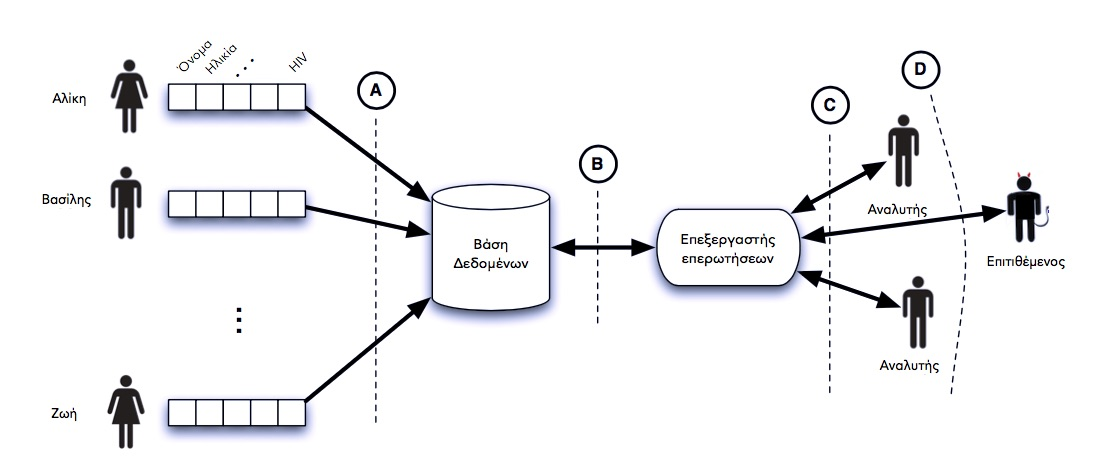
\includegraphics[width=\linewidth]{images/Hay.jpg}
  \caption{Στάδια ελέγχου ροής πληροφοριών}
  %\label{fig:boat1}
\end{figure}


Α. Διαταραχή εισόδου: Τα ίδια τα άτομα μπορούν να αλλοιώσουν τα δεδομένα που δίνουν στη βάση, προσθέτοντας θόρυβο. Με αυτόν τον τρόπο ο επιτιθέμενος δεν θα είναι ποτέ σίγουρος οτι οι ευαίσθητες πληροφορίες για κάποιο άτομο είναι σωστές, ενώ τα στατιστικά που συγκεντρώνουν οι αναλυτές δεν υφίστανται αξιόλογη μεταβολή.

Β. Μετασχηματισμός δεδομένων: Η αρχική βάση δεδομένων αναδομείται σε μια νέα εξυγιασμένη βάση στην οποία οι ευάισθητες πληροφορίες για συγκεκριμένα άτομα δεν είναι πια διακριτές. Σε αυτό το επίπεδο εφαρμόζεται το μοντέλο της \textlatin{k-anonymity}.

\textlatin{C}. Διαταραχή απάντησης επερωτήσεων: Οι αναλυτές μπορούν να επεξεργαστούν τα δεδομένα αλλά για να διασφαλιστεί η ιδιωτικότητα έχει προστεθέι θόρυβος. Εδώ εφαρμόζεται το μοντέλο της Διαφορικής Ιδιωτικότητας.

\textlatin{D}. Έλεγχος Πρόσβασης: Η βάση δεν είναι δημοσίως διαθέσιμη και μόνο οι έμπιστοι ερευνητές έχουν πρόσβαση. Έτσι αποτρέπεται η διαρροή ευαίσθητων δεδομένων σε κακόβουλα άτομα.





\subsection{Διατήρηση ποιότητας}

Όπως είναι προφανές, η απόκρυψη και η γενίκευση των δεδομένων έχει ως αποτέλεσμα την αλλοίωση της πληροφορίας και την απώλεια της αποτελεσματικότητας. Είναι γεγονός ότι το ποσό ανωνυμίας που έχει μια βάση δεδομένων είναι αντιστρόφως ανάλογο με την ποιότητα:

Η δημοσίευση της βάσης δεδομένων στο ακέραιο παρέχει την καλύτερη ποιότητα, ενώ η πλήρης απόκρυψη την καλύτερη ιδιωτικότητα. \textlatin{\cite{Sweeney:2001:CDC:935675}}
\begin{center}
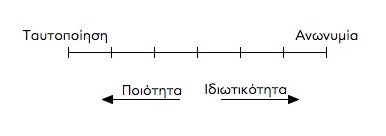
\includegraphics[scale=0.6]{images/Tension.jpg}
\end{center}
Κανένα από τα δυο άκρα δεν είναι επιθυμητό να προσεγγίζεται απο ένα σύνολο δεδομένων. Αφενός διότι στο ένα δεν θα παρέχεται καμία ασφάλεια στις εγγραφές και αφετέρου διότι στο άλλο τα δεδομένα θα είναι τόσο διαταραγμένα, που η ανάλυση θα είναι αδύνατη. Στο πλαίσιο της εργασίας αυτής θα συγκρίνουμε στο δυνατόν τις τεχνικές ιδιωτικότητας ως προς την ισορροπία που διατηρούν μεταξύ της προστασίας των εγγραφών και της τελικής ποιότητας των δεδομένων που παρέχονται στον αναλυτή. 


\section{Σκοπός}

Η παρούσα διπλωματική εργασία έχει τους εξής στόχους:
\begin{itemize}
\item Παρουσίαση τεχνικών και μεθοδολογιών που χρησιμοποιούνται για την ενίσχυση της ιδιωτικότητας στις βάσεις δεδομένων.
\item Επισκόπηση και κριτική αξιολόγηση από την σκοπιά της ασφάλειας και ιδιωτικότητας των υπό εξέταση προτάσεων/μεθοδολογιών.
\item Ανάδειξη κρίσιμων και ανοικτών ζητημάτων, καθώς και κατάδειξη προοπτικών για περαιτέρω έρευνα.
\end{itemize}


\section{Δομή Εργασίας}

Η εργασία είναι δομημένη ως εξής:

Στο δεύτερο κεφάλαιο παρουσιάζονται τα βασικά στοιχεία του προβλήματος. Γίνεται παρουσίαση και ανάλυση της μεθόδου \textlatin{k}-ανωνυμία 
(\textlatin{k-anonymity}). 
Δίνονται παραδείγματα και εξετάζονται οι αδυναμίες που την χαρακτηρίζουν. Στη συνέχεια, παρουσιάζονται δυο τεχνικές βελτιστοποίησης της μεθόδου της $k$-ανωνυμίας , η $l$-διαφορετικότητα (\textlatin{l-diversity}) και η $t$-εγγύτητα (\textlatin{t-closeness}). Αναλύεται η δυνατότητα και το κόστος εφαρμογής τους και εξετάζονται τα μειονεκτήματα χρήσης τους.

Στο τρίτο κεφάλαιο γίνεται θεμελίωση και ανάλυση του μοντέλου της Διαφορικής Ιδιωτικότητας. Δίνονται παραδείγματα, αναλύεται η επίδοσή των μηχανισμών και εξετάζεται η χρησιμότητα τους. 

Στο τέταρτο κεφάλαιο περιγράφονται αλγόριθμοι ανωνυμοποίησης που χρησιμοποιούν κυρίως τις τεχνικές γενίκευσης από το δεύτερο κεφάλαιο.

Στο πέμπτο κεφάλαιο αναπτύσσονται αλγοριθμικές εφαρμογές που υλοποιούν τα μοντέλα της Διαφορικής Ιδιωτικότητας. 

Στο έκτο κεφάλαιο συνοψίζονται τα αποτελέσματα της διπλωματικής εργασίας, αναφέρονται πιθανά ανοιχτά ζητήματα  καθώς επίσης και η προοπτική για περαιτέρω έρευνα. 

\clearpage


\section{\textlatin{Ralated Work}}

\subsection{ \textlatin{Blockchain}}

Η τεχνολογία \textlatin{Blockchain} είναι ένα από τα δημοφιλέστερα ζητήματα των τελευταίων ετών και έχει ήδη αρχίσει να αλλάζει τον τρόπο ζωής της σύγχρονης κοινωνίας εξ' αιτίας της επιρρόης της σε επιχειρήσεις και βιομηχανίες. Παρ'όλο που η τεχνολογία αυτή είναι ευρέως γνωστό ότι παρέχει αξιόπιστες υπηρεσίες, τα θέματα ασφάλειας και οι προκλήσεις πίσω από αυτή την καινοτόμο μεθόδο είναι κάτι που δεν πρέπει να μας εφησυχάζει.

Το μοντέλο \textlatin{blockchain} δεν εκφράζει μια απλή τεχνική, αλλά έναν συνδιασμό κρυπτογραφικών, μαθηματικών, αλγορίθμικών και οικονομικών μεθόδων, πάνω σε \textlatin{peer-to-peer} δίκτυα, που στοχεύουν στην επίλυση παραδοσιακών κατανεμημένων προβλημάτων συγχρονισμού σε βάσεις δεδομένων. Τα βασικά στοιχεία που χαρακτηρίζουν το μοντέλο είναι η αποκέντρωση, λόγω της μη χρήσης  κεντρικών εξυπηρετητών, η διαφάνεια, το \textlatin{open source} λογισμικό, η αδυναμία μεταβολής των εγγραφών και η ανωνυμία.

Κάθε εγγραφή που δημιουργείται από έναν κόμβο σε ένα δίκτυο του μοντέλου \textlatin{blockchain}, αφού ελεγχθεί για την εγκυρότητα της, τοποθετείται σε ένα \textlatin{block} μαζί με άλλες εγγραφές. Κάθε \textlatin{block} επισφραγίζεται με ένα «\textlatin{Proof of Work}», υπολογισμένο από έναν από τους κόμβους του δικτύου μέσω μιας συνάρτησης κατακερματισμού η οποία συνδυάζει στοιχεία του τρέχοντος \textlatin{block} αλλά και του προηγουμένου. Στη συνέχεια συνδέεται στην «αλυσίδα». Με αυτόν τον τρόπο καθίσταται αδύνατη η παραβίαση κάποιου \textlatin{block}, εκτός αν οι επιτιθέμενοι κατέχουν την πλειοψηφία της υπολογιστικής ισχύς των κόμβων του δικτύου.

Πέραν αυτής της υποθετικής κατάστασης, γνωστή και ως «51\% \textlatin{attack}», που θα έβαζε σε κίνδυνο την αλυσίδα\textlatin{\cite{bastiaan2015preventing}}, πρόσφατες έρευνες έχουν αναδείξει αρκετά θέματα ασφάλειας στα \textlatin{blockchain}. Ένα από τα σημαντικότερα είναι το \textlatin{Hard/Soft Fork}, που περιγράφει την  εμφάνιση προβλημάτων από την μη ταυτόχρονη αναβάθμιση λογισμικού των κόμβων.

Δεν υπάρχει αμφιβολία ότι το μοντέλο \textlatin{blockchain} είναι ένα κρίσιμο θέμα της εποχής. Όσο το χρησιμοποιούμε και επωφελούμαστε των δυνατοτήτων του, τόσο πρέπει να επιφυλασόμαστε και να εξετάζουμε πιθανά θέματα ασφάλειας που θα προκύπτουν.


\subsection{\textlatin{Cloud Privacy}}

Οι υπηρεσίες νέφους έχουν μπει για τα καλά στη ζωή μας, αφού οι απαιτήσεις χώρου, χρόνου και ταχύτητας συνεχώς αυξάνονται. Πολλές εταιρίες Πληροφορικής και οργανισμοί προσφέρουν αλλά και χρησιμοποιούν εφαρμογές και υπηρεσίες νέφους, μια τεχνολογία η οποία κατα κύριο λόγο χρησιμοποιεί υπολογιστές και εξυπηρετητές ενός δικτύου για την μεταφορά, την επεγεργασία και την αποθήκευση των δεδομένων.

Όπως σε κάθε νέα τεχνολογία, έτσι και στο \textlatin{Cloud Computing} παρουσιάζονται αρκετά θέματα αφαλείας, ένα από τα σημαντικότερα είναι η προστασία των δεδομένων. Οι οργανισμοί δεν πρόκειται να μεταφέρουν τα δεδομένα τους σε απομακρυσμένους εξυπηρετητές αν δεν λάβουν εγγύηση για προστασία των δεδομένων από τους παρόχους υπηρεσιών νέφους. 

Πολλές τεχνικές προστασίας έχουν διατυπωθεί για την προστασία των δεδομένων, αλλά υπάρχουν ακόμα ανοιχτά ζητήματα. Οι πιό δημοφιλείς μέθοδοι περιλαμβάνουν χρήση \textlatin{SSL} κρυπτογράφισης, συστήματα ανίχνευσης εισβολών και έλεγχο πρόσβασης βασισμένο σε \textlatin{Multi Tenancy}.
 % Introduction

\chapter{Ανεπάρκεια Προστασίας των Δεδομένων}

Οι εργασίες για την προστασία των προσωπικών δεδομένων έχουν ξεκινήσει εδώ και αρκετές δεκαετίες. Δυστυχώς, παρά τον σχετικά ορθό σχεδιασμό τους και το μεγάλο μέγεθος των συνόλων δεδομένων που αυτές εφαρμόζονται, η αποκάλυψη και η ταυτοποίηση εγγραφών είναι όπως θα δούμε αναπόφευκτη. 

Στο κεφάλαιο αυτό αναφέρουμε αρχικά περιπτώσεις διαρροής πληροφοριών κατά την επεξεργασία συνόλων δεδομένων. Στη συνέχεια, περιγράφουμε τη λειτουργία βασικών τεχνικών προστασίας και τονίζουμε τα σημεία στα οποία αυτές αποτυγχάνουν.



\section{Παραδείγματα αποκάλυψης πληροφορίας}

Κατά καιρούς έχουν προταθεί αρκετοί, διαφορετικοί μεταξύ τους, ορισμοί για την έννοια της διαρροής και αποκάλυψης πληροφοριών κατά την επεξερασία δεδομένων. 
Η αποκάλυψη σχετίζεται με την απόδοση σημαντικών πληροφοριών σε έναν ερωτώμενο, είτε πρόκειται για ένα άτομο είτε για έναν οργανισμό. Διακρίνουμε τρία είδη αποκάλυψης: όταν το άτομο μπορεί να ταυτοποιηθεί από το σύνολο δεδομένων (αποκαλυψη ταυτότητας), όταν διαρρεύσουν ευαίσθητες πληροφορίες για κάποιο άτομο (αποκάλυψη γνωρίσματος), και όταν τα δημοσιευμένα δεδομένα καθιστούν δυνατό τον ακριβέστερο προσδιορισμό της τιμής κάποιου γνωρίσματος μιας εγγραφής από ό, τι θα ήταν εφικτό (επαγωγική αποκάλυψη).


Παρακάτω κάνουμε μια συλλογή παραδειγμάτων αποκάλυψης και επιθέσεων στα οποία βλέπουμε πως από ένα σύνολο δεδομένων απο το οποίο απουσιάζουν ή αποκρύπτονται προσωπικά στοιχεία, ο επιτιθέμενος καταφέρνει να εξάγει την απαραίτητη πληροφορία ώστε να μπορεί να ταυτοποιηθεί τουλάχιστον ένα άτομο, ή η τιμή ενός ευαίσθητου γνωρίματος μιας εγγραφής, εντός του συνόλου. Τις περισσότερες φορές αυτό γίνεται με τη χρήση βοηθητικών πληροφοριών. Αυτό μπορεί να είναι οποιαδήποτε πρόσθετη πληροφορία που έχει πρόσβαση ο επιτιθέμενος, συμπεριλαμβανομένων παλαιότερων εκδόσεων της αρχικής βάσης δεδομένων. 


\begin{itemize}
   
\item \textbf{Η διαρροή δεδομένων αναζήτησης της $AOL$}\\
Τον Αύγουστο του 2006, η \textlatin{AOL Research} δημοσιεύει σε μια από τις ιστοσελίδες της έναν συμπιεσμένο φάκελο ο οποίος περιείχε 20 εκατομμύρια επερωτήσεις από 650.000 χρήστες. Σε μια προσπάθεια διατήρησης της ιδιωτικότητας, αντικατέστησαν τα ονόματα χρηστών με έναν αριθμό που δημιουργήθηκε τυχαία, ενώ επίσης επεξεργάστηκαν προσεκτικά αποκαλυπτικές επερωτήσεις (παράδειγμα, όταν τα άτομα αναζητούν το δικό τους όνομα ή αριθμό ασφαλείας). Ωστόσο, μπορούσε να εξαχθεί το πλήρες ιστορικό αναζήτησης ενός ατόμου. Αυτό με τη σειρά του, επέτρεπε σε οποιονδήποτε να εντοπίζει τα άτομα με βάση το ιστορικό αναζήτησης και, συνεπώς, να παραβιάσει την ιδιωτικότητά τους. 
Συγκεκριμένα, ερευνητές της \textlatin{New York Times} κατάφεραν να εντοπίσουν ένα άτομο από τα δημοσιευμένα και ανώνυμα αρχεία αναζήτησης, διασταυρώνοντάς τα με λίστες τηλεφωνικών καταλόγων.
Η \textlatin{AOL} αναγνώρισε το λάθος της και αφαίρεσε τα δεδομένα την αμέσως επόμενη ημέρα. Ωστόσο, η ζημιά είχε ήδη γίνει. Τα δεδομένα αναδιανεμήθηκαν από άλλους και μπορούν ακόμη και σήμερα να μεταφορτωθούν από \textlatin{mirror sites}.
\begin{figure} [h!]
\begin{center}
  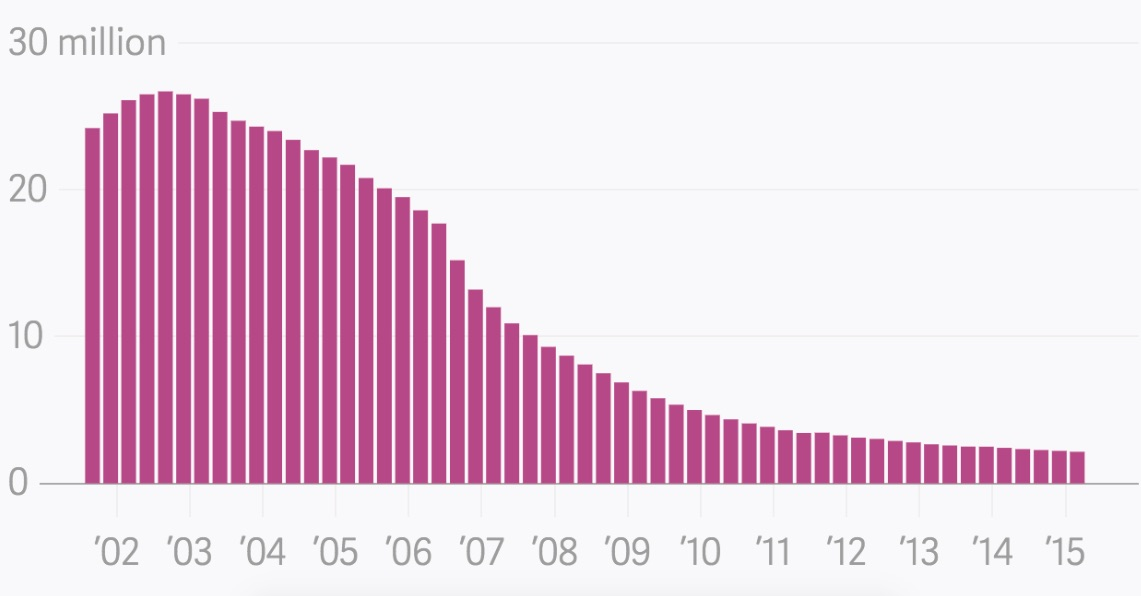
\includegraphics[scale=0.3]{images/AOL.jpg}
  \caption{Χρήστες $AOL$ από το 2002}
  %\label{fig:boat1}
  \end{center}
\end{figure}


Εντούτοις, δεν είναι σωστό να θεωρούμε ότι η προστασία της ιδιωτικότητας ενός συνόλου δεδομένων είναι δύσκολο έργο, επηρεασμένοι από το παραπάνω γεγονός. Αυτό συνέβει επειδή δεν δόθηκε ουσιαστική προσοχή στην ανωνυμοποίηση των αποτελεσμάτων αναζήτησης, πράγμα που συμπεραίνουμε από την άμεση απομάκρυνση από την εταιρία του υπευθύνου της κοινοποίησης των δεδομένων. Επιπλέον, ο προϊστάμενος της \textlatin{AOL Research} απολύεται ενώ ο \textlatin{CTO} παραιτήθηκε. Τελικά το γεγονός οδήγησε στην άμεση απομάκρυνση πολλών χρηστών, με αποτέλεσμα την επιτάχυνση της ήδη φθίνουσας πορείας της εταιρίας. 


\item \textbf{Διασταύρωση ιατρικών δεδομένων }

Μιά από τις δημοφιλέστερες αναδείξεις παραβίασης είναι η ταυτοποίηση του κυβερνήτη της Μασαχουσέτης σε λίστα ιατρικών δεδομένων. 

Είναι αποδεδειγμένο ότι το 63\% του πληθισμού των Ηνωμένων Πολιτειών μπορεί να ταυτοποιηθεί αν είναι γνωστά μόνο: ο ταχυδρομικός κώδικας, το φύλο και η ημερομηνία γέννησης ενός ατόμου. Σύμφωνα με ένα άρθρο \textlatin{\cite{Sweeney:2001:CDC:935675} }, αν ασκηθεί επίθεση συνδεσιμότητας σε δύο βάσεις δεδομένων που μοιράζονται αυτή την τριάδα γνωρισμάτων, τότε μπορεί να ταυτοποιηθεί μια τουλάχιστον εγγραφή. Συγκεκριμένα, στο πείραμα χρησιμοποιήθηκε ως πρώτη βάση ο κατάλογος ψηφοφόρων του \textlatin{Cambridge} και ως δεύτερη η βάση δεδομένων υγείας του \textlatin{ Massachusetts Group Insurance Commission (GIC)}. Τόσο ο κατάλογος ψηφοφόρων όσο και η βάση δεδομένων υγείας κάνουν χρήση των γνωρισμάτων \{ T.K, φύλο, ημερομηνία γέννησης \}, και αφού συνδυάστηκαν δυο εγγραφές, μια σε κάθε βάση, ταυτοποιήθηκαν τα στοιχεία του πρώην κυβερνήτη \textlatin{William Weld}. 

\begin{figure} [h!]
\begin{center}
  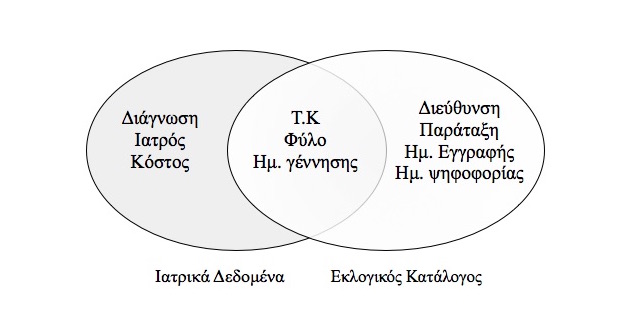
\includegraphics[scale=0.55]{images/TK.jpg}
  \caption{Συνδιασμός κοινών γνωρισμάτων}
  %\label{fig:boat1}
  \end{center}
\end{figure}

Αυτό που προκάλεσε ανησυχία δεν είναι το ότι κάτάφερε να ταυτοποιηθεί ένα διάσημο πρόσωπο συνδυάζοντας τα στοιχεία δυο βάσεων, αλλά ότι τέτοιου τύπου βάσεις, κυρίως με ιατρικά δεδομένα, είχαν ήδη διαμοιραστεί σε εταιρίες και ερευνητές πιστεύοντας λανθασμένα ότι τα δεδομένα είναι ανωνυμοποιημένα. 
Παρόλο που τα σύνολα δεδομένων δεν περιείχαν προσωπικά αναγνωριστικά, όπως το όνομα ή τον αριθμό κοινωνικής ασφάλισης ενός ασθενούς, τα άτομα μπορούσαν ακόμα να αναγνωριστούν συνδυάζοντας δύο βάσεις δεδομένων. 
\clearpage




\item \textbf{Το βραβείο του 1 εκατομμυρίου της  \textlatin{Netflix}}

Η \textlatin{Netflix} είναι μια εταιρία που παρέχει συνδρομιτικές υπηρεσίες τηλεόρασης σε μορφή \textlatin{on demand}. Για να βελτιώσει τον αλγόριθμο εμφάνισης προτεινόμενων ταινιών, η εταιρία δημοσίευσε αρχικά ένα σύνολο δεδομένων που περιείχε περισσότερες από 100 εκατομμύρια βαθμολογίες ταινιών από 480 χιλιάδες χρήστες σε σχεδόν 18 χιλιάδες τίτλους, και στη συνέχεια προσέφεραν ένα βραβείο αξίας 1 εκατομμυρίου δολαρίων σε εκείνους που θα μπορούσαν να βελτιώσουν το τρέχων σύστημα κατά τουλάχιστον 10\%.
Σε μια προσπάθεια διασφάλισης της ιδιωτικότητας των χρηστών τους, αφαιρούν δεδομένα προσωπικού χαρακτήρα.
Το μόνο που απομένουν είναι οι βαθμολογίες (βαθμολογία μεταξύ 1 και 5), η ημερομηνία που δόθηκε η βαθμολογία, το ανώνυμο αναγνωριστικό του χρήστη που έδωσε την αξιολόγηση και τέλος ο τίτλος της ταινίας που αξιολογήθηκε.
Η \textlatin{Netflix} δήλωσε επίσης ότι το σύνολο που δημοσιεύθκε αποτελούσε λιγότερο από το ένα δέκατο του πλήρους συνόλου δεδομένων και ότι τα δεδομένα είναι διαταραγμένα. 
Επίσης δήλωσε, ότι αυτό το ποσοστό επιλέχτηκε τυχαία.
Στην πραγματικότητα, αν παρατηρήσουμε το πλήθος βαθμολογιών για κάθε χρήστη βλέπουμε ότι ελάχιστοι έχουν βαθμολογήσει κάτω από 20 ταινίες \textlatin{\cite{Narayanan:2008:RDL:1397759.1398064}}. 

\begin{figure} [h!]
\begin{center}
  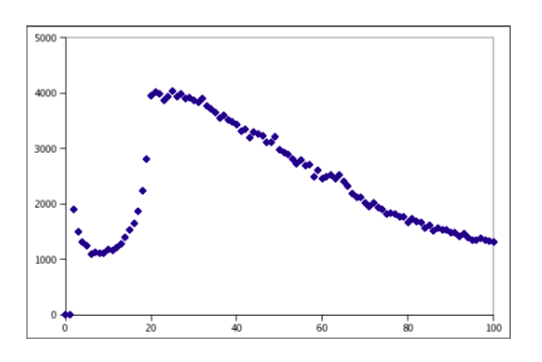
\includegraphics[scale=0.6]{images/Netflix.jpg}
  \caption{Πληθος χρηστών \textlatin{Netflix}, προς πλήθος βαθμολογιών}
  %\label{fig:boat1}
  \end{center}
\end{figure}

Επιπλέον, τέθηκε υπό αμφισβίτηση η υποτιθέμενη διάταραξη των δεδομένων, όταν ταυτοποιήθηκαν δυο συνδρομητές εντός των δεδομένων. O ένας από αυτούς είχε τροποποιημένες 1 από τις 306 αξιολογήσεις ενώ ο άλλος είχε 5 από 229, άρα το ποσοστό θορύβου ήταν ελάχιστο. 
Εδώ βέβαια, είναι σημαντικό να ληφθεί υπόψη ότι το σύνολο δεδομένων δημοσιέυτηκε με σκοπό την ανάπτυξη βελτιωμένων αλγορίθμων. Επομένως αν υπήρχε υπερβολική διαταραχή, θα είχε μειωθεί σημαντικά η χρησιμότητα του συνόλου. 

Το άρθρο του \textlatin{Narayanan} αποδεικνύει ότι απαιτείται ελάχιστη συνδεσιμότητα με εξωτερικά στοιχεία ώστε να ταυτοποιηθεί ένας συνδρομητής. Η σύνδεση στην προκειμένη περίπτωση γίνεται με εγγραφές από την βάση δεδομένων του \textlatin{IMDb}. Μέσα από μόνο 50 εγγραφές, ταυτοποιήθηκαν δυο χρήστες. 

Είναι εύλογο να αναρωτηθεί κάποιος για το αν αξίζει να ανησυχούμε για την ιδιωτικότητα δεδομένων τέτοιου τύπου. Αν όμως αναλογιστούμε το πόσο αποκαλυπτικό για τις πολιτικές πεποιθήσεις ενός ατόμου μπορεί να είναι η προτίμηση ταινιών όπως \textlatin{Fahrenheit 9/11} και \textlatin{Death by China}, συμπεραίνουμε ότι η παροχή προστασίας της ιδιωτικότητας είναι αναγκαία. 

\end{itemize}






\section{Ανεπαρκείς προσεγγίσεις προστασίας}

Ως κριτήρια της αποτελεσματικής ανωνυμοποίησης θωρούνται τα παρακάτω:
\begin{itemize}\label{kri}
\item Μη δυνατότητα εντοπισμού φυσικού προσώπου

\item Μη συνδεσιμότητα μεταξύ καταχωρήσεων που αντιστοιχούν σε ένα πρόσωπο

\item Μη δυνατότητα εξαγωγής συμπερασμάτων σχετικά με ένα φυσικό πρόσωπο.
\end{itemize}



Έχουν παρουσιαστεί κατα καιρούς αρκετές προτάσεις για τη διαφύλαξη της ιδιωτικότητας κατά την ανάλυση δεδομένων. Ωστόσο, οι περισσότερες από αυτές δεν ικανοποιούν τις παραπάνω εγγυήσεις απορρήτου. Αξίζει όμως να αναφερθούν αυτές οι προσπάθειες, διότι οφείλουμε να τονίσουμε ότι η διατήρηση της ιδιωτικότητας μπορεί να είναι ένα δύσκολο έργο με απροσδόκητα προβλήματα.

\begin{itemize}
   
\item \textbf{Επερωτήσεις μεγάλων συνόλων}\\
Μια κοινή ιδέα είναι να απαγορευτεί η εκτέλεση επερωτήσεων σχετικά με ένα συγκεκριμένο άτομο ή ένα μικρό σύνολο ατόμων. Είναι εύκολο να καταλάβουμε ότι αυτή η στρατηγική είναι ανεπαρκής όταν γνωρίζουμε ότι ένα συγκεκριμένο άτομο $X$ είναι στη βάση δεδομένων. Αυτό που μπορούμε να κάνουμε είναι να εφαρμόσουμε δυο «μεγάλες» επερωτήσεις. Η πρώτη, για παράδειγμα, μπορεί να είναι «Πόσα άτομα στη βάση δεδομένων έχουν διαβήτη?» και η δεύτερη «Πόσα άτομα στη βάση δεδομένων, που δεν ονομάζονται $X$, έχουν διαβήτη?». Από τα αποτελέσματα των δυο επερωτήσεων μπορούμε να συμπεράνουμε την κατάσταση του ατόμου $X$. Παρόλο που και οι δυο επερωτήσεις θεωρούνται μεγάλες, παραβιάστηκε η ιδιωτικότητα μιας εγγραφής.

\item \textbf{Έλεγχος Επερωτήσεων}\\
Μια άλλη στρατηγική είναι η αξιολόγηση κάθε επερώτησης στη βάση δεδομένων στο πλαίσιο του ιστορικού των επερωτήσεων, ώστε να προσδιοριστεί εάν μια απάντηση θα ήταν αποκαλυπτική. Εάν η επερώτηση θεωρηθεί ότι παραβιάζει την ιδιωτικότητα, απορρίπτεται και δεν επιστρέφεται απάντηση. Αυτή η μέθοδος μπορεί να χρησιμοποιηθεί για την ανίχνευση της επερώτησης στο προγούμενο παράδειγμα με το αν ένα άτομο Χ έχει ή όχι διαβήτη. Παρόλο που η τεχνική αυτή μπορεί να φαίνεται πολλά υποσχόμενη, η παρακολούθηση όλων των επερωτήσεων είναι υπολογιστικά ανέφικτη \textlatin{\cite{kleinberg1998segmentation}}. Επιπλέον, η ίδια η άρνηση απάντησης σε μιά επερώτηση μπορεί να είναι αποκαλυπτική. Για αυτούς τους λόγους, η παραπάνω προσέγγιση είναι πρακτικά μη εφαρμόσιμη.

\item \textbf{Δειγματοληψία}\\
Η δειγματοληψία μερικές φορές θεωρείται ως πιθανή λύση στο πρόβλημα. Εδώ ένας τυχαίος αριθμός εγγραφών στη βάση δεδομένων θα επιλεγεί τυχαία και οι πληροφορίες τους θα επιστραφούν προς ανάλυση. Ιδιότητες και στατιστικά στοιχεία μπορούν στη συνέχεια να υπολογιστούν στο νέο. Αν γίνει επιλογή ενός αρκετά μεγάλου υποδείγματος τα αποτελέσματα είναι αντιπροσωπευτικά της βάσης ως σύνολο.

Λαμβάνοντας υπόψη ότι το υποσύνολο είναι συνήθως μικρό σε σύγκριση με το μέγεθος της βάσης δεδομένων, είναι απίθανο να επιλεγεί μια συγκεκριμένη εγγραφή. Ωστόσο, κάθε φορά που επιλέγεται η ιδιωτικότητα της παραβιάζεται. Αυτό δεν είναι αποδεκτό, δεδομένου ότι θέλουμε να προστατεύσουμε την ιδιωτικότητα κάθε ατόμου στη βάση δεδομένων. Οπότε και πάλι αυτή η προσέγγιση δεν είναι εφαρμόσιμη σε πραγματικές καταστάσεις.

\item \textbf{Τυχαία Απάντηση (\textlatin{Randomized Response})}\\
Η προσέγγιση αυτή αποτελεί μια ισχυρή τεχνική παροχής ιδιωτικότητας. 
Εδώ τα δεδομένα τυχαιοποιούνται πριν αποθηκευτούν και τα στατιστικά στοιχεία μπορούν να υπολογιστούν από τα τυχαίοποιημένα δεδομένα. Η μέθοδος της τυχαίας απάντησης λειτουργεί με την ρίψη ενός νομίσματος, και με βάση το αποτέλεσμα η επερώτηση απαντάται αληθώς ή τυχαίως. Η ιδιωτικότητα είναι εγγυημένη λόγω της αβεβαιότητας ως προς τον τρόπο ερμηνείας μιας δεδομένης τιμής.

Αυτή η μέθοδος δημιουργήθηκε για καταστάσεις όπου τα άτομα δεν εμπιστεύονται τον υπεύθυνο/διαχειριστή δεδομένων. Η πιθανότητα επιστροφής τυχαίων δεδομένων επιλέγεται έτσι ώστε κατά τον υπολογισμό των στατιστικών στοιχείων για όλα τα δεδομένα που επιστρέφονται, το σφάλμα να παραμένει εντός ενός αποδεκτού διαστήματος. Ενώ η τυχαία απάντηση παρέχει προστασία της ιδιωτικότητας, το μειονέκτημα είναι ότι μπορεί να εισάγει παραπάνω θόρυβο στα δεδομένα και έτσι η προσέγγιση αυτή καθίσταται αδύνατη για σύνθετα δεδομένα.


\item \textbf{Τυχαίο Αποτέλεσμα  (\textlatin{Randomized Output})}\\
Κατά την μέθοδο αυτή προστίθεται θόρυβος στην έξοδο. Αυτό διαφέρει από την προηγούμενη τεχνική επειδή εκεί τα δεδομένα είναι τυχαιοποιημένα, ενώ σε αυτή την περίπτωση ο διαχειριστής έχει πρόσβαση στα αρχικά δεδομένα. Σε αυτή την τεχνική αυτός είναι που θα προσθέσει τυχαίο θόρυβο στο αποτέλεσμα των επερωτήσεων. 

Σημειώνουμε ότι αν γίνει αόριστα η παραπάνω προσέγγιση θα αποτύχει. Για παράδειγμα, ας υποθέσουμε ότι ο θόρυβος έχει μέση τιμή μηδέν και ότι χρησιμοποιείται ανεξάρτητη τυχαία συχνότητα για τη δημιουργία κάθε απάντησης. Σε αυτήν την περίπτωση, αν η ίδια επερώτηση δωθεί αρκετές φορές οι απαντήσεις μπορούν να αθροίζονται, να υπολογισθεί ο μέσος όρος και η αληθινή απάντηση θα αποκαλυφθεί τελικά.


\end{itemize}





Παρατηρούμε λοιπόν ότι οι παραπάνω προτάσεις προστασίας των δεδομένων αδυνατούν τελικά να διαφυλάξουν την ιδιωτικότητα των εγγραφών ενός συνόλου. Πάνω στις αδυναμίες αυτές στηρίζονται, όπως θα δούμε στη συνέχεια, οι μέθοδοι γενίκευσης, οι οποίες προσδίδουν σε ικανοποιητικό βαθμό τις επιθυμητές εγγυήσεις απορρήτου. 



















 % Background Theory 

\chapter{Μηχανισμοί γενίκευσης και ομαδοποίησης}

Οι μέθοδοι γενίκευσης αποτελούν την πιο ευρέως διαδεδομένη τεχνική ανωνυμοποίσης. Η συγκεκριμένη προσέγγιση συνίσταται στην ομαδοποίηση των εγγραφών ή την αλλοίωση των γνωρισμάτων στα οποία ανφέρονται τα δεδομένα, μέσω της τροποποίησης της αντίστοιχης κλίμακας μεγέθους. Παρόλο που αυτή η μέθοδος μπορεί να αποβεί αποτελεσματική για την πρόληψη του εντοπισμού ενός προσώπου, δεν εξασφαλίζει αποτελεσματική ανωνυμοποίηση σε όλες τις περιπτώσεις. Για αυτό το λόγο έχουν παρουσιαστεί ειδικές και τεχνολογικά εξελιγμένες ποσοτικές προσεγγίσεις για την πρόληψη του συνδιασμού συνόλων δεδομένων, προς εξαγωγή συμπερασμάτων για μεμονομένα φυσικά πρόσωπα. 

Το κεφάλαιο αυτό ξεκινά με την παρουσίαση  του μοντέλου της $k$-ανωνυμίας. Στη συνέχεια περιγράφονται οι τεχνικές της $l$-διαφορετικότητας και $t$-εγγύτητας που επεκτείνουν της δυνατότητες της $k$-ανωνυμίας. Τέλος γίνεται  παρουσίαση σύγχρονων αλγορίθμων ανωνυμοποίησης που υλοποιούν αυτές τις μεθόδους.

\section{Θεμελείωση}

Όπως είδαμε στις προηγούμενες παραγράφους, μια από τις αποδοτικότερες λύσεις για την προστασία της ιδιωτικότητας των δεδομένων, αλλά ταυτόχρονα διατήρηση της χρησιμότητάς τους, είναι η ανωνυμοποίηση. Παρακάτω δίνουμε μερικούς ορισμούς και προτάσεις που θα χρησιμοποιήσουμε κατά την διάρκεια της διαδικασίας αυτής.

\begin{definition}-Περι συνόλων δεδομένων-
\begin{itemize}
\item Ένα \textbf{σύνολο δεδομένων}(\textlatin{dataset})  είναι μια πεπερασμένη συλλογή στοιχείων.

\item Κάθε στοιχείο του, ή εγγραφή, είναι μια διατεταγμένη λίστα τιμών και αντιστοιχεί σε ένα πρόσωπο, στο οποίο αναφέρονται τα δεδομένα τιμών για κάθε \textbf{γνώρισμα}(\textlatin{attribute}).

Το σύνολο δεδομένων το μοντελοποιούμε σαν μια πλειάδα στοιχείων-γραμμών $D=(x_1,x_2,...,x_n)$.



\item Η ανωνυμοποιημένη προβολή του $D$ συμβολίζεται ως $R$.
\item Ορίζουμε ως $A=A_1,A_2,...,A_r$ μια συλλογή από $r$ \textbf{γνωρίσματα}.
\item Συμβολίζουμε ως $t$ κάθε πλειάδα στο $R$.
\item Κάθε $t[A_i]$ με $i \in [1,r]$ εκφράζει την τιμή του γνωρίσματος $A_i$ στο $R$ για την $t$.
\item Συμβολίζουμε  $t[A]=(t[A_1],t[A_2],...,t[A_r])$.
\end{itemize}
\end{definition}
Θεωρητικά, ως ανωνυμοποίηση ενός συνόλου δεδομένων $D$ θεωρείται ένα σύνολο γενικέυσεων των γνωρισμάτων του, αποτελούμενο από μια ακριβώς γενίκευση ανά γνώρισμα του $D$. Αυτές οι γενικεύσεις μετασχηματίζουν το $D$ σε ένα νέο σύνολο δεδομένων $D'$. Επιπλέον, η διαδικασία της γενίκευσης είναι αυτή που δίνει το όνομά της στην οικογένεια μεθόδων που αναλύουμε στη συνέχεια.








\section{\textlatin{k}-ανωνυμία}
\label{sec:k}

Η μέθοδος της $k$-ανωνυμίας\footnote{\textlatin{k-anonymity}} είναι μια μη διαδραστική\footnote{Με τον όρο μη διαδραστική τεχνική εννοούμε ότι, μετά την εφαρμογή της, δημοσιοποιείται μια εξυγιασμένη προβολή της βάσης} τεχνική ιδιωτικότητας 
. Αρχικά, η $k$-ανωνυμία θεωρήθηκε ως πιθανή λύση στο πρόβλημα της ιδιωτικότητας, κυρίως λόγω της εννοιολογικής απλότητας και των αποτελεσματικών αλγορίθμων που εγγυώνται την εφαρμογή της. Δυστυχώς προέκυψε άμεσα ότι έχει ελλείψεις και δεν είναι σε θέση να προστατεύσει την ιδιωτικότητα όλων των ατόμων. Θα αναλύσουμε την μέθοδο της $k$-ανωνυμίας και στη συνέχεια, αφού δούμε τα κενά ασφαλείας, θα παρουσιάσουμε βελτιώσεις.

Η ιδέα πίσω από την $k$-ανωνυμία είναι ότι όταν δίνονται πληροφορίες για ένα άτομο από μια εξωτερική πηγή, όπως το όνομά του, η ημερομηνία γέννησής, ο ταχυδρομικός κώδικας, το φύλο κλπ., θα πρέπει να είναι αδύνατο να βρεθεί, με ακρίβεια, στο ανωνυμοποιημένο σύνολο-πίνακα η γραμμή-πλειάδα που αντιστοιχεί στο άτομο αυτό \textlatin{\cite{k}}. Διαισθητικά, η διαδικασία πρέπει να έχει ως αποτέλεσμα οποιοσδήποτε χρήστης της βάσης να μην είναι σε θέση να αποκτήσει πληροφορίες σχετικά με ένα συγκεκριμένο άτομο, αφού δεν μπορεί να εντοπίσει τις πληροφορίες του στη βάση δεδομένων. Αυτό μπορεί να επιτευχθεί με την κατάργηση ορισμένων γνωρισμάτων σε συνδυασμό με την τροποποίηση ορισμένων τιμών πριν την απελευθέρωση της βάσης δεδομένων.

Το πρώτο βήμα κατά τη δημιουργία της ανώνυμης βάσης δεδομένων $R$, είναι η κατάργηση γνωρισμάτων που προσδιορίζουν σαφώς τα άτομα. Είναι αυτά που συνήθως χρησιμοποιούμε ως πρωτεύοντα κλειδιά \footnote{\textlatin{primary keys}}: Γνωρίζοντας την τιμή ενός γνωρίσματος κάποιου ατόμου μας διευκολύνει να βρούμε, με μεγάλη πιθανότητα, την πλειάδα που αντιστοιχεί σε αυτό το άτομο, παραδείγματος χάρη η διεύθυνση, ο αριθμός δελτίου ταυτότητας, το όνομα, το τηλέφωνο, κλπ. Ωστόσο, υπάρχουν γνωρίσματα τα οποία, όταν λαμβάνονται μαζί, είναι δυνατό να ταυτοποιηθεί ένα άτομο. Μια τέτοια συλλογή γνωρισμάτων ονομάζεται \textlatin{quasi-identifier}. Σε γενικές γραμμές, ένα \textlatin{quasi-identifier} περιέχει γνωρίσματα τα οποία είναι πιθανόν να υπάρχουν και σε άλλες βάσεις.

Ο ακριβής ορισμός ενός \textlatin{quasi-identifier}\footnote{Σε διάφορα ελληνικά άρθρα έχει χρησιμοποιηθεί ο όρος «ψευδοαναγνωριστικό σύνολο», που είναι εμφανώς μακρυά από την αγγλική έννοια} βασίζεται στον διαχωρισμό μεταξύ ευαίσθητων και μη ευαίσθητων γνωρισμάτων. Η τιμή ενός ευαίσθητου γνωρίσματος πρέπει να παραμείνει μυστική, πράγμα που σημαίνει ότι σε μια ανωνυμοποιημένη βάση δεδομένων θα πρέπει να είναι αδύνατο να συνδεθεί μια ευαίσθητη τιμή (συγκεκριμένα, μια πλειάδα που περιέχει μια ευαίσθητη τιμή) σε ένα συγκεκριμένο άτομο. Με αυτόν τον τρόπο είναι αδύνατο να μάθει κανείς την ευαίσθητη τιμή ενός ατόμου από την ανωνυμοποιημένη βάση δεδομένων και έτσι διατηρείται η ιδιωτικότητα. Όλα τα γνωρίσματα εκτός των ευαίσθητων θα ονομάζονται μη ευαίσθητα. Θεωρείται επίσης ότι τα επιλεγμένα ευαίσθητα χαρακτηριστικά δεν εμφανίζονται σε άλλες βάσεις δεδομένων. Επομένως, όταν είναι γνωστή η τιμή ενός ευαίσθητου γνωρίσματος, δεν είναι δυνατόν να βρεθεί το άτομο που αντιστοιχεί σε αυτήν την τιμή, πράγμα που σημαίνει επίσης ότι ένα ευαίσθητο γνώρισμα δεν περιλαμβάνεται ποτέ σε ένα \textlatin{quasi-identifier}. Καταλήγουμε στο συμπέρασμα ότι ένα \textlatin{quasi-identifier} αποτελείται μόνο από μη ευαίσθητα γνωρίσματα.

\begin{definition}(\textlatin{quasi-identifier})\\
Ένα σύνολο από μη ευαίσθητα γνωρίσματα $Q={Q_1,Q_2,...,Q_r}$ καλείται \textlatin{quasi-identifier} για μια βάση δεδομένων $D$ αν υπάρχει $t \in D$ ώστε η πρόταση
$$ t=t' \lor t[Q]\neq t[Q'] $$ για κάθε $t'\in D$ να είναι ψευδής.
\end{definition}

Με άλλα λόγια, υπάρχει τουλάχιστον μια εγγραφή στην αρχική βάση δεδομένων που μπορεί να προσδιοριστεί μοναδικά χρησιμοποιώντας μόνο τιμές γνωρισμάτων του συνόλου $Q$. Δηλώνουμε το σύνολο όλων των \textlatin{quasi-identifier} με το σύμβολο $QI$.

Είναι προφανές ότι αν ένα γνώρισμα μπορεί να ορισθεί ως πρωτεύον κλειδί, τότε αποτελεί ένα \textlatin{quasi-Identifier}, όπως επίσης συλλογές γνωρισμάτων όπως \{ημερομμηνία γέννησης, Τ.Κ., φύλο\}. 

Στην συνέχεια θα αναφερθούμε σε ομάδες ατόμων τα οποία θα έχουν ίδιες τιμές για ένα σύνολο από \textlatin{quasi-identifiers}.

\begin{definition}(Κλάση Ισοδυναμίας)\\
Μια κλάση ισοδυναμίας για έναν πίνακα $R$ σε σχέση με τα γνωρίσματα στο $A$ είναι ένα σύνολο πλειάδων $E=\{t_1,t_2,...,t_i\} \in R$ για τα οποία $t_1[A]=t_2[A]=...=t_i[A]$. 
\end{definition}
Δηλαδή, η προβολή κάθε πλειάδας επί των γνωρισμάτων στο Α είναι ακριβώς ίδια.



\begin{figure} [h!]
\begin{center}
  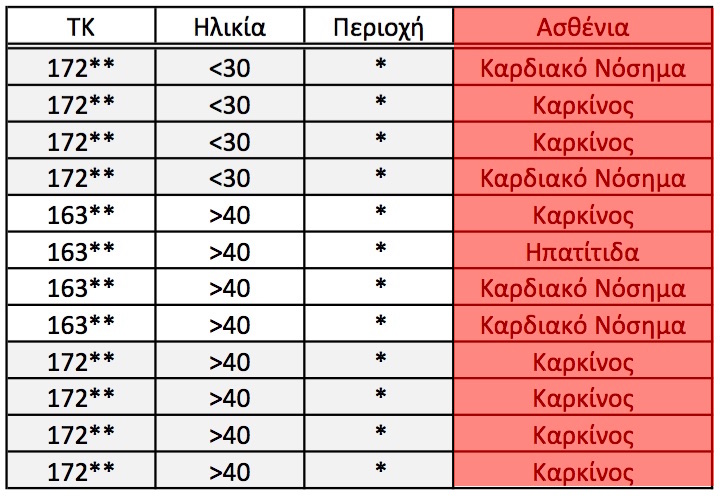
\includegraphics[scale=0.36]{images/k-anon.jpg}
  \caption{Ένα 4-ανώνυμο σύνολο δεδομένων}
  %\label{fig:boat1}
  \end{center}
\end{figure}

Στον παραπάνω πίνακα έχουμε 4 γνωρίσματα από τα οποία το ένα είναι ευαίσθητο (Ασθένια). Τα στοιχεία είναι ανωνυμοποιημένα. Επεμβαίνοντας στην Περιοχή και στα δυο τελευταία ψηφία του ΤΚ παρατηρούμε ότι δημιουργούνται τρεις ισοδύναμες κλάσεις, οι οποίες περιέχουν 4 εγγραφές οι κάθε μία.

Η $k$-ανωνυμία λειτουργεί εξασφαλίζοντας ότι υπάρχουν τουλάχιστον $k-1$ άλλα άτομα (δηλ. γραμμές στη βάση δεδομένων) που έχουν τις ίδιες τιμές για όλα τα \textlatin{quasi-identifiers}. Αυτό θα πρέπει να διασφαλίζει ότι αν ψάχνουμε για ένα συγκεκριμένο άτομο, θα έχουμε πάντα τουλάχιστον $k$ αποτελέσματα και έτσι δεν μπορούμε να προσδιορίσουμε την συγκεκριμένη πλειάδα.

\begin{definition}($k$-ανωνυμία)\\
Μια προβολή $R$ της βάσης $D$ θα είναι $k$-ανώνυμη αν για κάθε πλειάδα $t\in R$, και για κάθε \textlatin{quasi-identifier} $A\in IQ$, υπάρχουν τουλάχιστον $k-1$ άλλες πλειάδες $t_1,...,t_{k-1} \in R$ ώστε $t_1[A]=t_2[A]=...=t_{k-1}[A]$.
\end{definition}

Μια τεχνική για την επίτευξη $k$-ανωνυμίας είναι η γενίκευση γνωρισμάτων, η οποία αντικαθιστά τις τιμές των \textlatin{quasi-identifiers} με τιμές που είναι λιγότερο συγκεκριμένες αλλά σημασιολογικά ορθές. Ως αποτέλεσμα, περισσότερες εγγραφές θα έχουν το ίδιο σύνολο τιμών γνωριμάτων. Παρατηρούμε ότι ο παραπάνω πίνακας είναι 4-ανώνυμος, ενώ έχουμε \textlatin{quasi-identifier} το σύνολο γνωρισμάτων \{ΤΚ, Ηλικία, Περιοχή\}. Ο ορισμός της $k$-ανωνυμίας προϋποθέτει ότι ο υπεύθυνος της βάσης είναι σε θέση να αναγνωρίσει με ακρίβεια τα \textlatin{quasi-identifiers}. Ωστόσο, το έργο αυτό είναι πολύ δύσκολο στην εφαρμογή και είναι εύκολο να γίνει λάθος. Ειδικά ο διαχωρισμός ευαίσθητων και μη ευαίσθητων γνωρισμάτων μπορεί να είναι προβληματικός. Αυτό είναι σαφώς ένα από τα μειονεκτήματα της $k$-ανωνυμίας: Η υπόθεση ότι κάποιος είναι με ακρίβεια ικανός να βρει όλα τα \textlatin{quasi-identifiers} μοιάζει να είναι υπερβολικά απαιτητική.

\subsection{Επίτευξη \textlatin{k-anonymity}}

Υπάρχουν δυο κοινώς χρησιμοποιούμενες μεθόδοι για την επίτευξη της $k$-ανωνυμίας: 
\begin{itemize}

\item Η πρώτη είναι η τεχνική γενίκευσης - \textlatin{generalization}, όπου μια τιμή για ένα γνώρισμα μετατρέπεται σε μια γενικότερη και πιθανώς «αφηρημένη» τιμή. Παραδείγματος χάρη η τιμή του γνωρίσματος ΤΚ, όπου λείπουν τα δυο τελευταία ψηφία. Η απώλεια πληροφορίας είναι αναγκαστικά το τίμημα που πρέπει να πληρώσουμε ώστε να επιτευχθεί ιδιωτικότητα. 

\item Η δεύτερη μέθοδος είναι αυτή της απόκρυψης - \textlatin{suppression}. Όπως ορίζεται από την ίδια τη λέξη, εδώ η πληροφορία αποκρύπτεται εντελώς. Παραδείγματος χάρη η τιμή του γνωρίσματος Περιοχή. Η μέθοδος της απόκρυψης μπορεί να θεωρηθεί και σαν εφαρμογή της γενίκευσης, στον μέγιστο δυνατό βαθμό για κάποιο γνώρισμα. 
\end{itemize}
Μπορούμε τώρα να διατυπώσουμε το πρόβλημα της επίτευξης $k$-ανωνυμίας ελαχιστοποιώντας ταυτόχρονα τον αριθμό των γενικέυσεων ή αποκρύψεων που εφαρμόζονται. Αυτό θα είχε ως αποτέλεσμα τον βέλτιστο ανώνυμο πίνακα, όπου το βέλτιστο σημαίνει ότι η πληροφορία έχει παραμορφωθεί στο ελάχιστο, και έτσι μπορεί να θεωρηθεί ως η πιο χρήσιμη ανώνυμοποιημένη βάση δεδομένων. Ακόμα κι αν περιορίζουμε το πρόβλημα μόνο στην καταστολή των τιμών, μπορούμε να αποδείξουμε ότι το πρόβλημα βελτιστοποίησης είναι \textlatin{NP-Hard \cite{meyerson2004complexity}}. Επομένως στην πράξη εφαρμόζονται μόνο αλγόριθμοι προσέγγισης. Παρακάτω θα δείξουμε ότι η $k$-ανωνυμία αποτυγχάνει να προστατεύσει από πολλαπλές, πιθανώς ανεξάρτητες, προβολές.

\subsection{Επιθέσεις κατά της \textlatin{k}-ανωνυμίας}

Ενώ το μοντέλο της $k$-ανωνυμίας αποτελεί θεμελειώδη έννοια πάνω στην προστασία των δεδομένων, δεν εξασφαλίζει απόλυτα την ιδιωτικότητα σε συγκεκριμένες επιθέσεις. Όπως έχει αποδειχθεί, η $k$-ανωνυμία δεν εγγυάται πλήρως την μη αποκάλυψη της τιμής ευαίσθητων γνωρισμάτων των εγγραφών. Σε πολλές περιπτώσεις στατιστικών ερευνών απαιτείται η δημοσίευση των τιμών ενός ευαίσθητου γνωρίσματος ως έχουν, οι οποίες προφανώς δεν επηρεάζονται από την εφαρμογή $k$-ανωνυμοποίησης. Θεωρείται ότι εφόσον δεν μπορεί να ταυτοποιηθεί ένα άτομο με μια πλειάδα, δεν μπορεί να προκύψει συμπέρασμα για την τιμή που αυτό λαμβάνει για ένα ευαίσθητο γνώρισμα. Μπορεί, ωστόσο, κάποιος να συμπεράνει την τιμή του ευαίσθητου γνωρίσματος μιας ή περισσοτέρων ομάδων πλειάδων. Αν επιπλέον υπάρχει η δυνατότητα συνδυασμού κάποιων τιμών του \textlatin{quasi-identifier} που γνωρίζει ο επιτιθέμενος με κάποιες από αυτές που εμφανίζονται, θα μπορούσε να συμπεράνει την κλάση ισοδυναμίας που ανήκει η εγγραφή και πιθανότατα πληροφορίες σχετικά με το ευαίσθητο γνώρισμα. 

Οι ακόλουθες δύο κατηγορίες επιθέσεων αναλύθηκαν κατά την παρουσίαση της $l$-διαφορετικότητας \textlatin{ \cite{machanavajjhala2006ell}}.

\begin{itemize}
    \item \textbf{Eπίθεση ομοιογένειας}\\
    Αποδεικνύεται ότι εάν δεν υπάρχει διαφοροποίηση στην τιμή των ευαίσθητων γνωρισμάτων, παραβιάζεται η ιδιωτικότητα της εγγραφής. Εάν ο αριθμός των πλειάδων υπερβαίνει κατά πολύ τις πιθανές τιμές των ευαίσθητων χαρακτηριστικών, αυτό μπορεί να είναι μια κοινή κατάσταση. Παρατηρώντας τον προηγούμενο πίνακα βλέπουμε ότι αν ο επιτιθέμενος γνωρίζει ότι το άτομο που αναζητά βρίσκεται στη βάση δεδομένων, ενώ ταυτόχρονα ξέρει ότι είναι πανω απο 40 ετών και τα τρία πρώτα ψηφία του Τ.Κ. είναι 172, συμπεραίνει με βεβαιότητα ότι το άτομο πάσχει από καρκίνο. Ενώ η ταυτότητα του ατόμου προστατεύεται (ο επιτιθέμενος δεν γνωρίζει ποιά πλειάδα αντιστοιχεί στο άτομο), προκύπτει αποκάλυψη τιμής του ευαίσθητου γνωρίσματος.
    
    \item \textbf{Επίθεση με πρότερη γνώση}\\
    Ο επιτιθέμενος μπορεί επίσης να έχει γνώση σχετικά με τη κατανομή των ευαίσθητων τιμών. Στο προηγούμενο παράδειγμα, αν ο επιτιθέμενος γνωρίζει ότι το άτομο που αναζητά βρίσκεται στη βάση, ενώ ταυτόχρονα ξέρει ότι είναι κάτω απο 30 ετών, τότε η πλειάδα που αντιστοιχεί βρίσκεται στην πρώτη κλάση ισοδυναμίας. Αν επιπλέον γνωρίζει ότι είναι αθλητικός τύπος και προσέχει τη διατροφή του, εύκολα συμπεραίνει ότι είναι απίθανο να πάσχει απο καρδιακό νόσημα, άρα το άτομο έχει, με μεγάλη πιθανότητα, καρκίνο.
\end{itemize}

Μπορούμε να αποτρέψουμε την επίθεση ομοιογένειας διασφαλίζοντας ότι υπάρχει αρκετή ποικιλομορφία στις ευαίσθητες τιμές. Η προστασία από πρότερη γνώση είναι σχεδόν αδύνατη. Μπορούμε, ωστόσο, να δυσκολέψουμε τον επιτιθέμενο: Εάν υπάρχει μεγαλύτερη ποικιλία στις τιμές των ευαίσθητων γνωρισμάτων, θα χρειαστεί περισσότερη γνώση για την ανάκτηση της ακριβούς τιμής.
\clearpage










\section{\textlatin{l}-Διαφορετικότητα}

Το μοντέλο της $l$-διαφορετικότητας επεκτείνει την τεχνική της $k$-ανωνυμίας, έτσι ώστε να διασφαλιστεί ότι είναι αδύνατη η εφαρμογή επιθέσεων εξαγωγής συμπερασμάτων, εξασφαλίζοντας ότι κάθε γνώρισμα θα έχει τουλάχιστον $l$ διαφορετικές τιμές για κάθε κλάση ισοδυναμίας. 

\begin{definition}(Εντροπία $l$-διαφορετικότητας)\\
Για μια κλάση ισοδυναμίας $E$, έστω το $S$ το πεδίο τιμών των ευαίσθητων γνωρισμάτων και το $Pr [E, s]$ ο λόγος των εγγραφών στο $E$ που έχουν ευαίσθητη τιμή $s$, τότε το $E$ είναι $l$-διαφορετικό αν:
$$-\sum_{s\in S}Pr[E,s]log(Pr[E,s])\geq log(l)$$

\end{definition}

\begin{definition}
Ένα σύνολο δεδομένων είναι $l$-διαφορετικό αν όλες οι ισοδύναμες κλάσεις είναι $l$-διαφορετικές.
\end{definition}

Μιά απλούστερη εκδοχή του ορισμού είναι ότι κάθε κλάση ισοδυναμίας θα πρέπει να έχει τουλάχιστον $l$ διαφορετικές τιμές για το ευαίσθητο γνώρισμα (Διακριτή $l$-διαφορετικότητα).



\begin{figure} [h!]
\begin{center}
  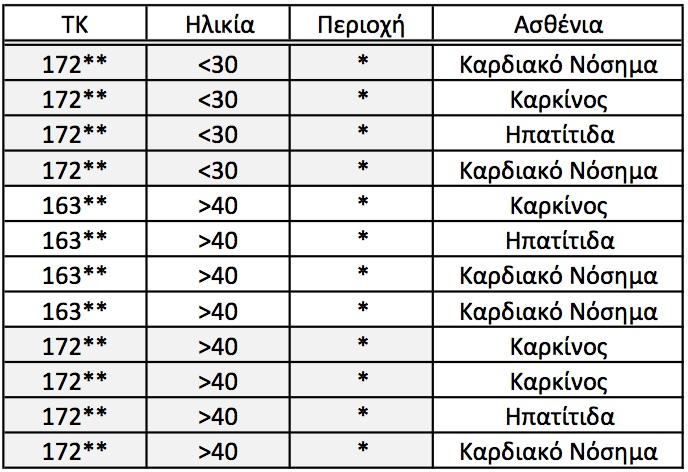
\includegraphics[scale=0.36]{images/k_anon.jpg}
  \caption{Ένα 3-διαφορετικό σύνολο δεδομένων}
  %\label{fig:boat1}
  \end{center}
\end{figure}

 Η σχέση στον ορισμό είναι σχεδόν η ίδια με την εντροπία του \textlatin{Shannon}, όπου οι πιθανότητες δίδονται τώρα ως κλάσματα συχνοτήτων των ευαίσθητων γνωρισμάτων. Όπως επισημάνθηκε στον παραπάνω ορισμό, για να υπάρχει $l$-διαφορετικότητα για κάθε κλάση ισοδυναμίας, η εντροπία ολόκληρου του πίνακα πρέπει να είναι τουλάχιστον $log (l)$. Κάποιες φορές αυτό μπορεί να είναι υπερβολικά περιοριστικό, καθώς η εντροπία ολόκληρου του πίνακα θα είναι αρκετά μικρή εάν κάποιες τιμές είναι πολύ συχνές. Αυτό οδηγεί στην ακόλουθη λιγότερο συντηρητική έννοια της $l$-διαφορετικότητας.
 
 \begin{definition}(Αναδρομική $(c,l)$-διαφορετικότητα)\\
 Έστω $m$ ο αριθμός των πιθανών τιμών ευαίσθητου γνωρίσματος σε μια κλάση ισοδυναμίας και $r_i$, με $i \in [1,m]$, το πόσες φορές η $i$-οστή συχνότερη τιμή εμφανίζεται στην κλάση $E$. Τότε η $E$ θα έχει $(c,l)$-διαφορετικότητα αν:
 $$r_1\leq c(r_l+r_{l+1}+...+r_m)$$
 \end{definition}
 
 
 \begin{definition}
Ένα σύνολο δεδομένων είναι $(c,l)$-διαφορετικό αν όλες οι ισοδύναμες κλάσεις είναι $l$-διαφορετικές.
\end{definition}
Η αναδρομική $(c, l)$-διαφορετικότητα εξασφαλίζει ότι η πιο συχνή τιμή δεν εμφανίζεται πολύ συχνά και οι λιγότερο συχνές τιμές δεν εμφανίζονται πολύ σπάνια.
 
 Γενικά, συμπεραίνουμε ότι η μέθοδος της $l$-διαφορετικότητας αντιμετοπίζει τις επιθέσεις ομοιογένειας, ενώ ταυτόχρονα δυσκολεύει τους επιτιθέμενους με πρότερη γνώση. Όσο υψηλότερη είναι η τιμή του $l$, τόσο περισσότερη γνώση απαιτείται για να αποκαλυφθεί η τιμή ενός ευαίσθητου χαρακτηριστικού ενός ατόμου. 
 
 
 
 \subsection{Επίτευξη \textlatin{l}-διαφορετικότητας}
 
 Η εισαγωγή της τεχνικής αυτής αποτελεί μια σημαντική βελτίωση της $k$-ανωνυμίας. Ωστόσο, παρατηρείται ιδιέταιρη δυσκολία στην εφαρμογή της.
 
 
 
 Ας θεωρήσουμε μια βάση δεδομένων μεγέθους $n=100000$ με ένα ευαίσθητο γνώρισμα δύο και μόνο πιθανών τιμών, το να έχει ή όχι τον ιό $HIV$. Έστω ότι το 99\% του δείγματος έχει την τιμή ΟΧΙ (είναι αρνητικοί στον ιό). Αν επιθυμούμε οποιαδήποτε τιμή προσέγγισης $l$-διαφορετικότητας, κάθε κλάση ισοδυναμίας θα πρέπει να έχει και τις δυο τιμές. Αυτό μεταφράζεται στην δημιουργία 1000 κλάσεων, που θα έχει ως αποτέλεσμα μεγάλη απώλεια πληροφορίας κατά την εφαρμογή γενίκευσης. Σημειώνουμε επίσης ότι επειδή η εντροπία του ευαίσθητου γνωρίσματος στον πίνακα είναι πολύ μικρή, η $l$-διαφορετικότητα μπορεί να επιτευχθεί μόνο εάν διαλέξουμε ένα αρκετά μικρό $l$, καθώς για μεγάλη τιμή θα ήταν στην πραγματικότητα αδύνατο να εξασφαλίσει διαφορετικότητα. Παρόλο που αυτό δεν αποτελεί ελάττωμα, το αναφέρουμε για να δείξουμε τη δυνητική δυσκολία να επιτύχουμε την $l$-διαφορετικότητα.
 
 \subsection{Επιθέσεις κατά της \textlatin{l}-διαφορετικότητας}
 
 Παρακάτω αναφέρουμε δυο είδη επιθέσεων κατά της μεθόδου αυτής.
 \begin{itemize}
     \item \textbf{Ασύμμετρη Επίθεση}\\
     Όταν η συνολική κατανομή είναι ασύμμετρη, η εφαρμογή $l$-διαφορετικότητας δεν εξασφαλίζει την μη αποκάλυψη τιμής ενός γνωρίσματος. Στο προηγούμενο παράδειγμα όπου το 99\% ενός πληθισμού έχει την τιμή ευαίσθητου γνωρίσματος ΟΧΙ, η αρχή της $l$-διαφορετικότητας επιτρέπει να υπάρχει μια κλάση ισοδυναμίας με ίσο αριθμό θετικών/αρνητικών στον ιό ατόμων. Παρατηρούμε ότι η ιδιωτικότητα κάθε ατόμου που ανήκει σε αυτή την κλάση χάνεται επειδή θεωρείται ότι έχει 50\% πιθανότητα να είναι θετικός στον ιό, αντί της πραγματικής 1\%.
     
     Ας θεωρήσουμε τώρα μια κλάση ισοδυναμίας που έχει 98 θετικές εγγραφές και μόνο 2 αρνητικές. Αυτή η κλάση είναι 2-διαφορετική και έχει μεγαλύτερη εντροπία από το σύνολο του πίνακα,   ικανοποιώντας έτσι κάθε $l$-διαφορετικότητα εντροπίας που κάποιος μπορεί να εφαρμόσει. Ωστόσο, ένα τυχαίο άτομο στην κλάση θα θεωρείται 98\% θετικός, αντί για 1\%. Στην πραγματικότητα, αυτή η κλάση ισοδυναμίας έχει ακριβώς την ίδια διαφορετικότητα με μια τάξη που έχει 2 θετικές και 98 αρνητικές εγγραφές, παρόλο που οι δύο κλάσεις παρουσιάζουν πολύ διαφορετικά επίπεδα κινδύνων ιδιωτικότητας.
     
     
     \item \textbf{Επίθεση ομοιότητας}\\
     Ένα άλλο πιθανό πρόβλημα παρουσιάζεται όταν οι τιμές ευαίσθητων χαρακτηριστικών είναι διακριτές αλλά σημασιολογικά παρόμοιες. Για παράδειγμα, μία κλάση ισοδυναμίας μπορεί να περιέχει διάφορους τύπους καρκίνων. Σε αυτή την περίπτωση γνωρίζουμε ότι όλοι στην ομάδα έχουν καρκίνο. Ένα άλλο παράδειγμα είναι ένα γνώρισμα που περιγράφει τον μισθό ενός συνόλου εργαζομένων. Κάθε άτομο σε μια κλάση μπορεί να έχει μια μοναδική τιμή, αλλά το συνολικό διάστημα μπορεί ακόμα να είναι μικρό. Ως εκ τούτου θα μπορούσαμε να μαντέψουμε με ακρίβεια το μισθό κάθε ατόμου λαμβάνοντας τον μέσο όρο στην κλάση.


 \end{itemize}









\clearpage
\section{\textlatin{t}-Εγγύτητα}

Μια βελτίωση της $l$-διαφορετικότητας που προσπαθεί να λύσει τα προβλήματα που παρουσιάσαμε ονομάζεται $t$-εγγύτητα. Εδώ προσπαθούμε να διασφαλίσουμε ότι η κατανομή ενός ευαίσθητου γνωρίσματος στην κλάση είναι ίδια με την κατανομή του σε ολόκληρο τον πληθυσμό. Αυτό έχει ως αποτέλεσμα τον ακόλουθο ορισμό.

\begin{definition}
Μια κλάση ισοδυναμίας $E$ θα έχει $t$-εγγύτητα εάν η απόσταση μεταξύ της κατανομής ενός ευαίσθητου γνωρίσματος στην κλάση αυτή και της κατανομής του γνωρίσματος σε ολόκληρο τον πίνακα δεν υπερβαίνει ένα κατώφλι $t$.
\end{definition}

\begin{definition}
Ένα σύνολο δεδομένων θα έχει $t$-εγγύτητα, αν όλες οι κλάσεις ισοδυναμίας του έχουν $t$-εγγύτητα.
\end{definition}

Το ακριβές μέτρο απόστασης που χρησιμοποιείται δεν έχει μεγάλη σημασία στο πλαίσιο της εργασίας αυτής. Παρόλο που η εγγύτητα είναι μια σαφής βελτίωση των προηγούμενων τεχνικών προστασίας της ιδιωτικότητας, θα δούμε στη συνέχεια ότι εξακολουθεί να είναι ευάλωτη σε μια επίθεση συνδεσιμότητας. Αυτό συμβαίνει κυρίως διότι η $t$-εγγύτητα - όπως επίσης kai οι προηγούμενες μέθοδοι - επικεντρώνονται σε στατικά δεδομένα που μένουν αμετάβλητα. Επομένως, περιορίζονται σε μια και μόνο δημοσίευση και δεν υποστηρίζουν την αναδημοσίευση μιας νέας προβολής της βάσης δεδομένων. 

Αυτό προκαλεί προβλήματα επειδή μπορεί να υπάρχει μια βάση δεδομένων, από διαφορετική εταιρία/οργανισμό, όπου είναι αποθηκευμένες σχεδόν οι ίδιες πληροφορίες.
Αν αυτός ο οργανισμός κοινοποιήσει μια ανώνυμοποιημένη βάση δεδομένων, η παραδοχή μιας «μοναδικής» δημοσίευσης παύει πλέον να ισχύει. Στην πραγματικότητα δηλαδή είναι αδύνατον να αποτρέψουμε πολλαπλές δημοσιεύσεις της ίδιας βάσης δεδομένων, και επομένως μηχανισμός ιδιωτικότητας που προυποθέτει μοναδική δημοσίευση, θεωρείται πρακτικά επισφαλής. 








\section{Επίθεση Τομής}

Μια επίθεση που δεν μπορεί να αντιμετοπίσει καμία από τις προαναφερθείσες τεχνικές, και ουσιαστικά καμία εκ των μεθόδων γενίκευσης, είναι η επίθεση τομής. 
Είναι μια ιδιαίτερη περίπτωση επίθεσης σύνθεσης, όπου συνδυάζονται δύο ή περισσότερες κοινοποιήσεις της βάσης δεδομένων ή επικαλυπτόμενες βάσεις, δημοσιευμένες από διαφορετικές οντότητες \textlatin{\cite{ganta2008composition}}. 
Η επίθεση τομής εξαρτάται από μια σημαντική ιδιότητα που μπορεί να διαθέτει ένας μηχανισμός προστασίας ιδιωτικότητας, εν ονόματει εντοπισμός (\textlatin{locatability}).

\begin{definition}(Εντοπισμός)\\
Έστω $Q$ το σύνολο των \textlatin{quasi-identifiers} τιμών μιας εγγραφής στην αρχική βάση δεδομένων $D$. Ένας μηχανισμός ανωνυμοποίησης $M$, που παράγει μια ανωνυμοποιημένη προβολή $R$ δεδομένης της βάσης $D$, ικανοποιεί την ιδιότητα του εντοπισμού αν κάποιος μπορεί να ταυτοποιήσει ένα σύνολο πλειάδων $\{t_1,t_2,...,t_k\}$ του $R$ που να αντιστοιχούν στο $Q$.
\end{definition}

Εν ολίγοις, δηλώνεται ότι, δεδομένων των τιμών των \textlatin{quasi-identifiers} ενός ατόμου, μπορούμε να βρούμε την κλάση ισοδυναμίας που ανήκει.

Όπως αναφέραμε και στην παράγραφο \ref{sec:k}, οι περισσότεροι αλγόριθμοι ανωνυμοποίησης παράγουν μια ανώνυμη βάση, δεδομένης την αρχικής. 
Η πλειοψηφία αυτών των μηχανισμών ικανοποιεί την ιδιότητα εντοπισμού, πράγμα που δεν ισχύει αναγκαστικά για όλους. 
Για αυτούς που δεν ικανοποιούν αυστηρά την ιδιότητα, τα πειράματα αποκαλύπτουν ότι απλές επιθέσεις συνδυαστικού τύπου μπορούν ακόμα να εντοπίσουν την κλάση ισοδυναμίας ενός ατόμου με ικανοποιητικού βαθμού πιθανότητα.
Η επίθεση τομής προϋποθέτει ότι ο μηχανισμός που χρησιμοποιείται για τη δημιουργία της ανώνυμης βάσης ικανοποιεί την ιδιότητα εντοπισμού.

Παρακάτω παρουσιάζουμε την αλγόριθμο της επίθεσης τομής:\\

\begin{algorithm}[H]
\textlatin{
 \KwData{$R_1,R_2,...,R_n$ \textgreek{Οι $n$ ανώνυμες προβολές}}
 $P$ \textgreek{ένα σύνολο ατόμων, κοινό στις $n$ δημοσιεύσεις}\\
 \For{i in P}{
  \For{j=1 to n}{
   $e_{ij} \longleftarrow GetEqClass(R_j,i)$\\
   $s_{ij} \longleftarrow SensitiveValueSet(e_{ij})$\\
   }{
   $S_i \longleftarrow s_{i1}\cap s_{i2} \cap ... \cap s_{in}$\\
  }
 }
 \Return $S_1, S_2,...,S_{|P|}$
 \caption{ Intersection Attack}}
\end{algorithm}

Έστω $R_1,R_2,...,R_n$ oι $n$ ανώνυμες προβολές μιας βάσης $D$. Έστω $P$ ένα επικαλυπτόμενο υποσύνολο ατόμων, των οποίων γνωρίζουμε την τιμή των 
\textlatin{quasi-identifiers}, που εμφανίζεται σε όλες τις δημοσιεύσεις.
Η συνάρτηση \textlatin{GetEqClass} επιστρέφει την κλάση ισοδυναμίας που ανήκει το άτομο, βασιζόμενη στις τιμές των \textlatin{quasi-identifiers} του.
Εφόσον υποθέσαμε ότι ο μηχανισμός προστασίας ιδιωτικότητας που παράγει τις ανωνυμοποιημένες προβολές $Rj$ ικανοποιεί την ιδιότητα εντοπισμού, αυτή η συνάρτηση υπάρχει σε κάθε περίπτωση.
Η συνάρτηση \textlatin{SensitiveValueSet} επιστρέφει το σύνολο των (ξεχωριστών) ευαίσθητων τιμών για τα άτομα σε μια δεδομένη κλάση ισοδυναμίας.

Αυτό που κάνει ο βρόχος είναι, από κάθε ανώνυμη προβολή να εξάγει το πιθανό σύνολο τιμών για το ευαίσθητο χαρακτηριστικό. Στη συνέχεια παίρνουμε την τομή όλων αυτών των συνόλων. Αν καταλήξουμε σε μία μόνο τιμή, μόλις αποκαλύψαμε το ευαίσθητο χαρακτηριστικό.

Έστω για παράδειγμα, ότι θέλουμε να εξάγουμε συμπέρασμα για την ασθένεια ενός ατόμου $a$, για το οποίο γνωρίζουμε ότι βρίσκεται στην ανωνυμοποημένη βάση $R$ και στην επίσης ανωνυμοποιημένη $B$. Έχουμε φτάσει στο συμπέρασμα με βάση την επεξεργασία της $R$,  ότι ο $a$ έχει Καρκίνο ή Διαβήτη, ενώ από την $B$, ότι πάσχει απο Καρδιακό νόσημα είτε από Καρκίνο. Προκύπτει λοιπόν το συμπέρασμα:

$$S_a={\{\text{Καρκίνος, Διαβήτης}\}}\cap \{\text{Καρδιά, Καρκίνος}\}=\{\text{Καρκίνος}\}$$

Προφανώς η ιδιωτικότητα του ατόμου $a$ έχει παραβιαστεί. Αυτή είναι μια «τέλεια παραβίαση» επειδή μπορούμε να συμπεράνουμε την ακριβή ευαίσθητη τιμή του ατόμου. Με άλλα λόγια ο επιτιθέμενος μαθαίνει την τιμή του ευαίσθητου γνωρίσματος ενός ατόμου με βεβαιότητα 100\%. Μια άλλη μορφή παραβίασης είναι η «μερική παραβίαση», η οποία μπορεί να συμβεί όταν ο επιτιθέμενος είναι σε θέση να συμπυκνώσει τις πιθανές ευαίσθητες τιμές σε λίγες μόνο, οι οποίες θα μπορούσαν να αποκαλύψουν πολλές πληροφορίες. 

Αν πάρουμε πάλι ως παράδειγμα την αποκάλυψη της ασθένειας του ατόμου $a$ και προκύψει μετά την τομή των αποτελεσμάτων:

$$S_a={\{\text{Υπέρταση, Ανεύρυσμα, Φλεβοθρόμβωση}\}}$$

προκύπτει το συμπέρασμα ότι το άτομο αυτό πάσχει από μια καρδιακή νόσο. Η πιθανότητα εύρεσης της νόσου σε αυτή την περίπτωση είναι 33\%.


Η επίθεση τομής εφαρμόστηκε σε δεδομένα ανωνυμοποιημένα με την μέθοδο της $k$-ανωνυμίας, $l$-διαφορετικότητας και $t$-εγγύτητας. Το συμπέρασμα ήταν ότι και οι τρεις μηχανισμοί αποτυγχάνουν να προστατεύσουν την ιδιωτικότητα όλων των ατόμων. Η $l$-διαφορετικότητα και η $t$-εγγύτητα αποδίδουν καλύτερα από την $k$-ανωνυμία, ωστόσο παρατηρούνται ακόμη περιπτώσεις παραβίασης. 
Κάτι που προκύπτει επιπλέον, είναι ότι για την $l$-διαφορετικότητα και $t$-εγγύτητα πρέπει να δημιουργηθούν μεγάλες κλάσεις ισοδυναμίας, με αποτέλεσμα μεγάλη απώλεια πληροφορίας.

Το συμπέρασμα λοιπόν είναι ότι όλες οι μεθόδοι γενίκευσης παρέχουν ικανοποιητική ιδιωτικότητα, προστατεύοντάς τα δεδομένα είτε από αποκάλυψη ταυτότητας, είτε από αποκάλυψη τιμής ευαίσθητου γνωρίσματος. Σε ιδιέταιρες καταστάσεις όμως, καμία από τις μεθόδους αυτές δεν μπορεί να αντιμετωπίσει την επίθεση τομής.

%Οι περισσότεροι μηχανισμοί ανωνυμοποίσησης που αναφέραμε στα προηγούμενα κεφάλαια έχουν εφαρμοστεί αλγοριθμικά




\clearpage
\section{Αλγόριθμοι Γενίκευσης}

Οι περισσότεροι μηχανισμοί ανωνυμοποίησης που παρουσιάσαμε στα προηγούμενα κεφάλαια, έχουν προσεγγιστεί κατά καιρούς με αλγορίθμους σε διάφορες γλώσσες προγραμματισμού, και έχουν αξιολογηθεί σε έρευνες. Στην παράγραφο αυτή επιδιώκουμε να συγκεντρώσουμε τις βέλτιστες και ταχύτερες προσεγγίσεις.

Τα τελευταία χρόνια έχουν δημοσιευτεί δεκάδες άρθρα που περιγράφουν και αναλύουν αλγορίθμους ανωνυμοποίσης συνόλων δεδομένων. 
Στόχος των αλγορίθμων αυτών είναι η δημιουργία μιας τροποποιημένης έκδοσης του συνόλου δεδομένων, έτσι ώστε η ιδιωτικότητα των εγγραφών να προστατεύεται επαρκώς, ενώ ταυτόχρονα, να διατηρείται η χρηστικότητα των δημοσιευμένων δεδομένων.



\subsection{\textlatin{Mondrian}}

Ο \textlatin{Mondrian} είναι ένας από τους κλασικότερους αλγορίθμους γενίκευσης και παρουσιάστηκε αρχικά ως εφαρμογή του μοντέλου της $k$-ανωνυμίας. Ως είσοδο δέχεται το σύνολο των αρχικών δεδομένων και επιστρέφει την βέλτιστη γενίκευση\footnote{Ως βλετιστη γενίκευση ορίζεται το ποσό γενίκευσης κατά το οποίο παρέχεται η μέγιστη δυνατή ιδιωτικότητα, εξασφαλίζοντας την ελάχιστη απώλεια πληροφορίας} του. 
Θεωρείται ένας από τους πιο σύγχρονους αλγορίθμους ανωνυμοποίησης και είναι ελκυστικός τόσο λόγω των λύσεων που παρέχει όσο και του χαμηλού χρόνου εκτέλεσης.

Η γενική ιδέα πίσω από τον αλγόριθμο είναι ένας \textlatin{top-down} διαχωρισμός των δεδομένων. Όλα τα αρχεία ανήκουν αρχικά στην ίδια κλάση ισοδυναμίας και αναδρομικά επιλέγεται μια διάσταση για να χωριστούν οι κλάσεις ισοδυναμίας, μέχρις ότου δεν υπάρχει καμία διάσταση στην οποία μπορεί να χωριστεί η κλάση για να παράγει έγκυρες $k$-ανώνυμες συστάδες. 

Ο αλγόριθμος ακολουθεί την εξής διαδικασία:
\begin{itemize}
    \item Ορίζονται οι περιοχές που καλύπτουν το χώρο των πεδίων τιμών  του \textlatin{quasi-identifier}
    \item Επιλέγεται η διάσταση με την οποία θα γίνει ο διαχωρισμός των κλάσεων. Υπάρχουν πολλοί τρόποι επιλογής, συνήθως όμως επιλέγεται η διάσταση με το μεγαλύτερο εύρος τιμών .
    \item Εφαρμόζεται ο διαχωρισμός κατά την παραπάνω επιλεγμένη διάσταση, βάσει της μέσης τιμής του αντίστοιχου γνωρίσματος, έτσι ώστε οι τιμές που είναι μικρότερες ή ίσες απο αυτήν να βρίσκονται στην αριστερή κλάση και οι υπόλοιπες να βρίσκονται στην δεξιά κλάση ισοδυναμίας.
    \item Η διαδικασία επαναλαμβάνεται για κάθε μία από τις δύο προκύπτουσες κλάσεις ισοδυναμίας αναδρομικά μέχρι να μην υπάρχει άλλη επιτρεπόμενη πολυδιάστατη τομή για διαχωρισμό σε καμία διάσταση. 
    \item Ως έξοδος, προκύπτει ο βέλτιστος διαχωρισμός και συνεπώς η κατάλληλη πολυδιάστατη γενίκευση που θα χρησιμοποιηθεί για να ανακωδικοποιηθούν τα δεδομένα.
\end{itemize}

Σε ψευδογλώσσα:


\begin{algorithm}[H]
\textbf{Συνάρτηση} $partition\_anon(P)$\\
\textlatin{
 \KwData{ \textgreek{Διαμ'εριση $P$}}
 \eIf{\textgreek{είναι αδύνατη περεταίρω πολυδιάστατη τομή της $P$}}{
   \Return $P$
   }{
   $dim \longleftarrow choosedimension(P)$\\
    $lhs \longleftarrow \{t\in \text{\textgreek{διαμεριση}}: t.dim = false\}$\\
     $rhs \longleftarrow \{t\in \text{\textgreek{διαμεριση}}: t.dim = true\}$\\
     \Return $partition\_anon(lhs)\cup partition\_anon(rhs)$
  }
 \caption{ Mondrian}}
\end{algorithm}



\subsection{Συσταδοποίηση (\textlatin{Clustering})}

Πέραν της χρήσης του $Mondrian$ για την ανωνυμοποίηση των δεδομένων, έχουν υιοθετηθεί μοντέλα από τον τομέα της εξόρυξης δεδομένων. Κλασικό παράδειγμα είναι η εφαρμογή αλγορίθμων συσταδοποίησης, η οποία θεωρείται πολλά υποσχόμενη μέθοδος.

Για την ανάπτυξη τέτοιων αλγορίθμων είναι απαραίτητο να ξεπεραστούν τα προβλήματα εγγύτητας με την αναζήτηση πλησιέστερων γειτόνων που χρησιμοποιεί κάθε φορά για να επιλέξει εγγραφές για συσταδοποίηση. Χρησιμοποιείται η εξής διαδικασία:
αντί να βρεθεί ο πλησιέστερος γείτονας μεταξύ όλων των εγγραφών, αρκεί να βρεθεί ο πλησιέστερος ανάμεσα σε κάποιο δείγμα ενός σταθερού αριθμού εγγραφών και να το δεχτεί. 



\subsection{ \textlatin{k - OPTIMIZE}}

Ο αλγόριθμος αυτός παρουσιάστηκε ως η βέλτιστη-ταχύτερη μέθοδος $k$-ανωνυμοποίησης.
Χρησιμοποιεί προτάσεις της Θεωρίας Γραφημάτων, ενω αποφεύγονται δαπανηροί αλγριθμικοί υπολογισμοί, όπως η ταξινόμηση \textlatin{\cite{Bayardo:2005:DPT:1053724.1054048}}.


Ο αλγόριθμος ξεκινά υπολογίζοντας μια τυχαία ανωνυμοποίηση του συνόλου. 
Στη συνέχεια εισέρχεται σε μια φάση γενίκευσης στην οποία οι τιμές αφαιρούνται διαδοχικά (πάντοτε επιλέγοντας εκείνη που βελτιώνει περισσότερο το χρονικό κόστος) έως ότου αυτό να μην μπορεί πλέον να βελτιωθεί.
Στη συνέχεια, μεταβαίνει σε μια φάση «εξειδίκευσης» στην οποία οι τιμές προστίθενται επαναληπτικά (και πάλι πάντα επιλέγοντας εκείνη που παρέχει τη μεγαλύτερη βελτίωση του κόστους) έως ότου δεν είναι δυνατή η βελτίωση. 
Ο αλγόριθμος εκτελεί επαναπληπτικά αυτές τις δύο φάσεις μέχρις ότου καμία φάση δεν είναι ικανή να βελτιώσει το \textlatin{score} (υποδηλώνοντας ότι επιτυγχάνεται τοπικό ελάχιστο).
Στο σημείο αυτό, καταγράφεται το κόστος ανωνυμοποίησης και ο αλγόριθμος επαναλαμβάνει ολόκληρη τη διαδικασία. Σημειώνεται ότι ο αλγόριθμος αυτός δεν έχει συνθήκες διακοπής και αντίθετα προσπαθεί συνεχώς να βελτιώσει την καλύτερη λύση που βρέθηκε μέχρι να σταματήσει ο χρήστης.






\begin{figure} [ht]
\begin{center}
  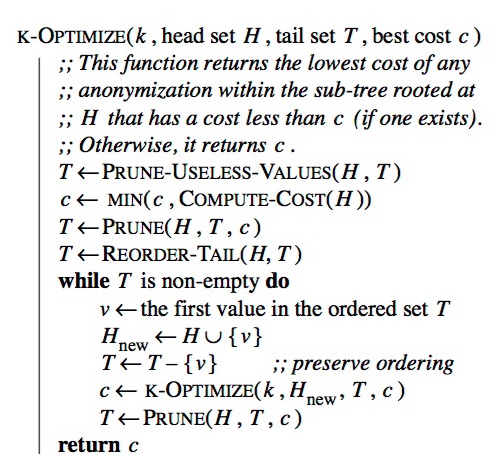
\includegraphics[scale=0.5]{images/optimize1.jpg}
  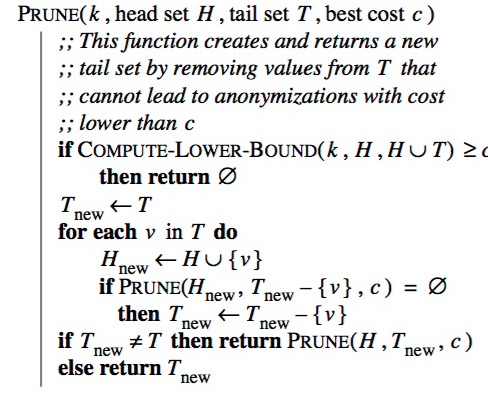
\includegraphics[scale=0.5]{images/optimize2.jpg}
  \caption{Μοντελοποίηση του αλγορίθμου \textlatin{k-optimize}  }
  %\label{fig:boat1}
  \end{center}
\end{figure}

Οφείλουμε να παρατηρήσουμε ότι αρκετοί από τους αλγορίθμους αυτούς χρησιμοποιούνται στην πράξη, ενώ διαθέσιμοι σε \textlatin{open-source} μορφή ύπάρχουν από πολλές πηγές, όπως \textlatin{Anonymization Toolbox}  από το Πανεπιστήμιο του Ντάλας και το \textlatin{ARX - Powerful Data Anonymization}, τα οποία υποστηρίζουν κυρίως τα μοντέλα $k$-ανωνυμίας και $l$-διαφορετικότητας. Στις βιβλιοθήκες ανωνυμοποίησης συνήθως συναντάμε και αλγορίθμους όπως ο \textlatin{Datafly} και ο \textlatin{Incognito}, οι οποίοι όμως δεν είναι τόσο αποτελεσματικοί όσο αυτοί που αναφέραμε παραπάνω.

Ένα βασικό σημείο στο οποίο υστερούν οι προαναφερθέντες αλγόριθμοι αποτελεί ο χρόνος εκτέλεσης, όπου κάποιες φορές είναι πιθανό να καθιστά αδύνατη την πρακτική εφαρμογή τους. Πρόσφατες μελέτες διερευνούν τη χρήση συμπληρωματικών μεθόδων ώστε να καταστούν οι μηχανισμοί αυτοί αποδοτικότεροι σε σχέση με την υπολογιστική τους πολυπλοκότητα, κάνοντάς τους φιλικότερους στη χρήση σε πρακτικές εφαρμογές. \textlatin{\cite{mohammadian2014fast}} % Experimental Setup

\chapter{Διαφορική Ιδιωτικότητα}

Στο προηγούμενο κεφάλαιο αναλύσαμε τεχνικές στις οποίες ο διαχειριστής του συνόλου δεδομένων δημοσιεύει μια εξυγιανσμένη εκδοχή τους. Ωστόσο, είδαμε ότι η ανωνυμοποίηση του συνόλου δεδομένων αρκετές φορές δεν επαρκεί για να προστατέψει τα δεδομένα από έναν ισχυρό και καλά προετοιμασμένο επιτιθέμενο. Σε μια βάση $n$ στοιχείων για παράδειγμα, ένας γνώστης συγκεκριμένου γνωρίσματος των $n-1$ αντικειμένων, μπορεί εύκολα να συμπεράνει την τιμή του γνωρίσματος του ατόμου που απομένει. 
Στη συνέχεια θα παρουσιάσουμε και θα αναλύσουμε την διαφορική ιδιωτικότητα, μια διαδραστική μέθοδο η οποία προστατεύει τα δεδομένα, ακόμη και από επιτιθέμενους με πρότερη γνώση.


\section{Η έννοια της διαδραστικότητας}

\begin{figure} [ht]
\begin{center}
  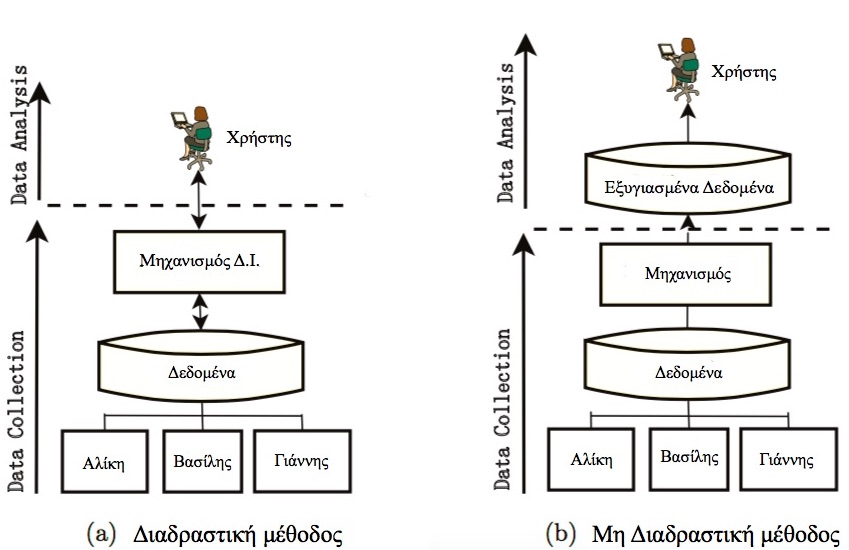
\includegraphics[scale=0.4]{images/Int.jpg}
  \caption{Η έννοια της διαδραστικότητας}
  %\label{fig:boat1}
  \end{center}
\end{figure}
Μία ελπιδοφόρα προσέγγιση που θα μπορούσε να καλύψει τα κενά των τεχνικών ομαδοποίησης που παρουσιάσαμε, είναι να μεσολαβίσει της πρόσβασης στη βάση δεδομένων μια αξιόπιστη διασύνδεση η οποία θα απαντάει τις επερωτήσεις των αναλυτών. 

Έχουν προταθεί κατα καιρούς αρκετές κρυπτογραφικές μέθοδοι, κυρίως μέσω προσθήκης θορύβου, ώστε να διασφαλιστεί η ιδιωτικότητα των μηχανισμών επερωτήσεων και να εξασφαλιστεί η ανώνυμη επικοινωνία Βάσης-Αναλυτή. Σε αυτό το σημείο όμως, είναι εύλογο το ερώτημα:

«Μήπως οι τιμές εξόδου των μηχανισμών αυτών, ήδη αποκαλύπτουν υπερβολικά πολλές πληροφορίες?» 



Μία λύση στο πρόβλημα αυτό είναι η τυχαιοποίηση των αποτελεσμάτων του μηχανισμού.
Υποθέστε ότι κάποιος θέλει να μάθει αν έχουμε  κάποιο συγκεκριμένο χαρακτηριστικό. Σε κάθε τέτοια ερώτηση απαντάμε με τον ακόλουθο τρόπο:

\begin{enumerate}
    \item Ρίχνουμε ένα νόμισμα
    \item Αν έρθει γράμματα, τότε απαντάμε αληθώς.
    \item Αν έρθει κορώνα, τότε ρίχνουμε ένα δεύτερο νόμισμα και απαντάμε «Ναι» αν έρθει κορώνα και «Οχι» αν έρθει γράμματα.
\end{enumerate}

Συμπεραίνουμε ότι δεν μπορεί να προκύψει ακριβές συμπέρασμα για το αν έχουμε ή όχι το χαρακτηριστικό. Αυτό το παράδειγμα παρουσιάζει έναν απλό μηχανισμό τυχαιοποίησης των αποτελεσμάτων των επερωτήσεων. Τον φορμαλισμό της σκέψης  αυτής έρχεται να εκφράσει η διαφορική ιδιωτικότητα.


\section{Θεμελίωση}

Πρωτού δώσουμε τον ορισμό της διαφορικής ιδιωτικότητας θα δούμε δύο ιδιότητες όπου κάθε μέθοδος ιδιωτικότητας οφείλει να κατέχει.

\textbf{Ανθεκτικότητα σε πρότερη γνώση}:

Στο εισαγωγικό παράδειγμα είδαμε ότι υπάρχει πιθανότητα για έναν επιτιθέμενο να έχει γνώση για όλα σχεδόν τα στοιχεία της βάσης. Γενικά οφείλουμε πάντα να λογαριάζουμε οποιαδήποτε πληροφορία μπορεί ήδη να γνωρίζει κάποιος για ένα υποσύνολο δεδομένων. Επειδή είναι πολύ δύσκολο να προσδιοριστεί ποσοτικά, υποθέτουμε ότι ιδανικά ο επιτιθέμενος γνωρίζει τα πάντα, εκτός από τις ατομικές πληροφορίες ενός ατόμου.



\textbf{Ανθεκτικότητα σε πολλαπλές εφαρμογές - Σύνθεση (\textlatin{composition}}):

Αν εφαρμόσουμε την μέθοδο αρκετές φορές σε συγγενείς βάσεις, ο επιτιθέμενος δεν επιτρέπεται να μπορεί να συνδυάσει τα αποτελέσματα ώστε να εξακριβώσει την ταυτότητα κάποιου ατόμου. Εκεί είναι που αποτυγχάνουν οι περισσότερες μη διαδραστικές τεχνικές. Θα αναλύσουμε περισσότερο την ιδιότητα αυτή μετά τον ορισμό της διαφορικής ιδιωτικότητας.




Έστω $x=(x_1,x_2,...,x_n)$ ένα σύνολο δεδομένων, και $x_i$ μια εγγραφή του.

\begin{definition}(Γειτνίαση)\\
Δύο σύνολα δεδομένων $x,x'$ \textbf{γειτνιάζουν}, αν για κάθε στοιχείο τους ισχύει
$ x_i=x'_i $ για κάθε $i\in [1,n]$, εκτός ένός το πολύ στοιχείου.
\end{definition}

Δηλαδή δυο γειτονικά σύνολα δεδομένων πρέπει να διαφέρουν το πολύ σε ένα στοιχείο τους. Συμβολίζουμε $x\sim x'$ 
\textlatin{\cite{dpc}}.

Όταν προτάθηκε για πρώτη φορά διαφορική ιδιωτικότητα , η σχέση γειτνίασης καθορίστηκε με έναν ελαφρώς διαφορετικό τρόπο: δύο βάσεις δεδομένων είναι γειτονικές εάν και μόνο εάν μια βάση δεδομένων είναι αποτέλεσμα της προσθήκης / αφαίρεσης ενός χρήστη από την άλλη βάση δεδομένων\textlatin{\cite{10.1007/11681878_14}}. 

Το κίνητρο πίσω από τον αρχικό ορισμό είναι να γίνει απόκρυψη της συμμετοχής οποιουδήποτε ατόμου στη βάση δεδομένων. Ένα τυπικό παράδειγμα είναι μια βάση δεδομένων για ασθενείς με συγκεκριμένο τύπο ασθένειας.
Ο ορισμός γενικεύει την αρχική έννοια της σχέσης γειτνίασης προκειμένου να χειριστεί βάσεις δεδομένων που αποτελούνται από αριθμητικές τιμές. Στην πραγματικότητα,  ο ορισμός αυτός μπορεί να επεκταθεί περαιτέρω για να ενσωματώσει πιο πολύπλοκα αντικείμενα, όπως διανυσματικά μεγέθη.

Τονίζουμε ότι η Διαφορική Ιδιωτικότητα είναι σε θέση να εγγυηθεί ότι το αποτέλεσμα υπολογισμών σε μια βάση δεδομένων δεν μεταβάλλεται πολύ όταν οποιοσδήποτε μεμονωμένος χρήστης στη βάση δεδομένων αλλάζει τις πληροφορίες του.
Με άλλα λόγια, η διατήρηση της ιδιωτικότητας είναι ισοδύναμη με την απόκρυψη αλλαγών στη βάση δεδομένων

\begin{definition} (Τυχαιοποιημένη συνάρτηση)\\
Έστω $X$ το σύνολο όλων των πεπερασμένων συνόλων δεδομένων και $B$ το σύνολο όλων των τυχαίων μεταβλητών με εικόνα Β. Ορίζουμε μια τυχαιοποιημένη συνάρτηση $M$:
$$M:X\longrightarrow  B $$
\end{definition}

Στη βιβλιογραφία συναντάμε την έννοια της τυχαιοποιημένης συνάρτησης και ως τυχαιοποιημένου αλγορίθμου ή μηχανισμου.

\begin{definition}(Διαφορική Ιδιωτικότητα)\\
Δεδομένου $\epsilon >0$, μια τυχαιοποιημένη συνάρτηση $M$ αποδίδει   
$\epsilon$-διαφορική ιδιωτικότητα, αν για κάθε ζεύγος συνόλων δεδομένων $x$, $x'$ με $x\sim x'$ και κάθε $S\subseteq R_M$, όπου $R_M$ το σύνολο τιμών της $M$, ισχύει:
$$ P[M(x)\in S]\leq e^{\epsilon} \cdot P[M(x')\in S]$$

\end{definition}

Ως $\epsilon$ θεωρούμε έναν μικρό, όχι αμελητέο, θετικό αριθμό, συνήθως στο διάστημα $(0.01,ln2)$. Όσο μικρότερη η τιμή του, τόσο μεγαλύτερη η προστασία των εγγραφών. Είναι προφανές ότι ο ορισμός παύει να είναι χρήσιμος αν $\epsilon < \frac{1}{n}$. Επίσης θεωρούμε το $n$ ως καθολικά γνωστή πληροφορία.

Παρατηρούμε ότι η σχέση μπορεί να γραφεί ισοδύναμα
$$ P[M(x')\in S]\leq e^{\epsilon} \cdot P[M(x)\in S]$$
εξ αιτίας της συμμετρίας που προκύπτει από τον ορισμό της γειτνίασης των βάσεων. Η έννοια της διαφορικής ιδιωτικότητας μας βεβαιώνει ότι ο επιτιθέμενος δεν μπορεί να συμπεράνει από την εικόνα της $M$, με μεγάλη πιθανότητα, αν τα δεδομένα από μια και μόνο εγγραφή έχουν μεταβληθεί. 

Σε ορισμένες περιπτώσεις είναι χρήσιμο να θεωρίσουμε μια γενίκευση του ορισμού:

\begin{definition}
Δεδομένου $\epsilon, \delta >0$, μια τυχαιοποιημένη συνάρτηση $M$ αποδίδει   
$(\epsilon,\delta)$-διαφορική ιδιωτικότητα, αν για κάθε ζεύγος συνόλων δεδομένων $x$, $x'$ με $x\sim x'$ και κάθε $S\subseteq R_M$, όπου $R_M$ το σύνολο τιμών της $M$, ισχύει:
$$ P[M(x)\in S]\leq e^{\epsilon} \cdot P[M(x')\in S]+\delta$$

\end{definition}

Προφανώς, όσο μεγαλύτερο είναι το $\delta >0$ τόσο πιο εύκολα ένας επιτιθέμενος μπορεί να ξεχωρίσει το ποια βάση είναι η $x'$ και ποιά η $x$. Ο αρχικός ορισμός (με $\delta =0$ δηλαδή) είναι ασφαλέστερος. Συνοπτικά, ο όρος δ αντιπροσωπεύει την πιθανότητα ότι μερικά άτομα μπορεί να συμβεί να χάσουν περισσότερη ιδιωτικότητα από ό, τι τα υπόλοιπα, ότι το πολλαπλασιαστικό φράγμα δεν ισχύει για όλους. Αν το δ είναι πολύ μικρό, ο κίνδυνος αυτός είναι πολύ μικρός.




\textbf{\textlatin{Counting Query}}: Ένας βασικός τύπος επερωτήσεων που θα εξετάσουμε εκτενώς είναι το \textlatin{counting query}, το οποίο καθορίζεται από μια δίτιμη απεικόνιση (\textlatin{predicate}) στις εγγραφές του συνόλου $q:X \longrightarrow \{0,1\}$, και γενικεύεται σε ολόκληρο το σύνολο δεδομένων $x \in X^n$, υπολογίζοντας τον λόγο των εγγραφών που ικανοποιούν την απεικόνιση: 
$$q(x)=\frac{1}{n}{\sum_{i=1}^{n} q(x_i)}$$



Όπως είδαμε και στο παράδειγμα της εισαγωγής, η ιδιωτικότητα δεν πρέπει να θεωρείται τετριμμένη ακόμη και αν δίνονται μόνο \textlatin{counting} επερωτήσεις στη βάση, επειδή τα αποτελέσματα μπορούν να συνδυαστούν με συνέπεια την αποκάληψη πληροφορίας για κάποια εγγραφή.

\begin{figure} [ht]
\begin{center}
  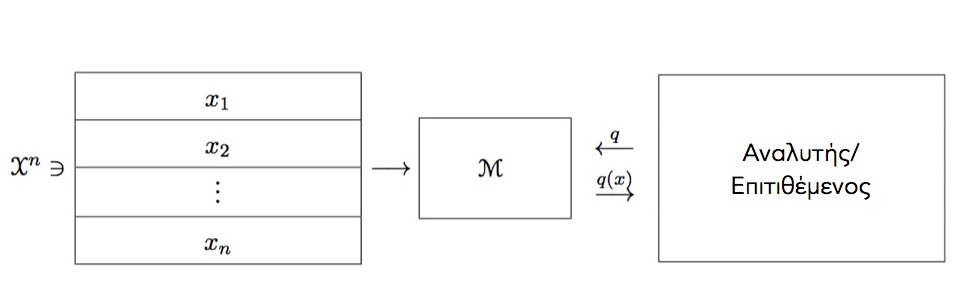
\includegraphics[scale=0.4]{images/M.jpg}
  \caption{Λειτουργία μηχανισμού ΔΙ}
  %\label{fig:boat1}
  \end{center}
\end{figure}



\subsection{Θεώρημα Σύνθεσης}

Στην εισαγωγή του κεφαλαίου αναφέραμε ότι η διαφορική ιδιωτικότητα χαρακτηρίζεται από δύο βασικές ιδιότητες. Αρχικά, εξασφαλίζει ότι τα αποτελέσματα θα είναι ανεπηρέαστα από οποιαδήποτε εξωτερική γνώση. Δεύτερον, η μέθοδος παρουσιάζει ανθεκτηκότητα στην μετεπεξεργασία. Όπως είδαμε, το αποτέλεσμα από την εφαρμογή ενός μηχανισμού ιδιωτικότητας κοινοποιείται, και εν συνεχεία αυτό μπορεί είτε να χρησιμοποιηθεί αυθαίρετα από άλλους είτε να χρησιμοποιηθεί ως δείγμα ώστε να εφαρμοστεί ένας νέομηχανισμός ακόμη και από τον ίδιο χρήστη. Η ανθεκτηκότητα στην επαναληπτική εφαρμογή μηχανισμών εγγυάται ότι δεν πρόκειται να χαθεί μέρος της ιδιωτικότητας, παρά την επαναχρησιμοποίηση\\
\textlatin{\cite{Dwork:2010:BDP:1917827.1918366}}.

\begin{theorem}\label{ak}(Σύνθεση)
 Έστω μηχανισμός $M:X\longrightarrow  B $ που παρέχει $\epsilon$-διαφορική ιδιωτικότητα. Τότε για κάθε συνάρτηση $f$, η σύνθεση $f\circ M$ διατηρεί $\epsilon$-διαφορική ιδιωτικότητα.
\end{theorem}

Στη συνέχεια εισάγουμε δυο κανόνες σύνθεσης που χρησιμοποιούνται συχνά για την δημιουργία νέων μηχανισμών ιδιωτικότητας. Ο νόμος της ακολουθιακής σύνθεσης παρουσιάζεται παρακάτω και χρησιμοποιείται συνήθως όταν απαιτείται ο υπολογισμός πολλών πληροφοριών από την ίδια βάση.


\begin{theorem} (Ακολουθιακή σύνθεση - \textlatin{sequential composition})\\
 Έστω μηχανισμός $M_1:X\longrightarrow  B $ που παρέχει $\epsilon_1$-διαφορική ιδιωτικότητα και μηχανισμός $M_2:X\longrightarrow  B $ που παρέχει $\epsilon_2$-διαφορική ιδιωτικότητα. Ορίζουμε νέο μηχανισμό $M(x)=(M_1(x),M_2(x))$, ο οποίος θα διατηρεί $(\epsilon_1+\epsilon_2)$-διαφορική ιδιωτικότητα.
\end{theorem}

Ας υποθέσουμε ότι έχουμε μια βάση δεδομένων με τους μισθούς μιας εταιρίας. Έστω ότι κάποιος θέλει να κοινοποιήσει την μέση τιμή, αλλά και την διακύμανση των μισθών. Θα χρησιμοποιήσει έναν μηχανισμό ιδιωτικότητας για τον μέσο και έναν για την διακύμανση, οι οποίοι στη συνέχεια μπορούν να συνδιαστούν δίνοντας την τάξη της ιδιωτικότητας που παρουσιάζεται στο θεώρημα. Τέλος, παρατηρούμε ότι το θεώρημα συνεπάγεται την εξής πρόταση:\textbf{ Όσο περισσότερες επερωτήσεις τίθενται στην ίδια βάση, τόσο περισσότερη ιδιωτικότητα χάνεται}.

Για συγκεκριμένες εφαρμογές που απαιτείται επαναχρησιμοποίηση, ο μηχανισμός που θα επιθυμούσαμε να σχεδιάσουμε είναι ένα αποτέλεσμα «προσαρμοστικής» σύνθεσης διάφορων μηχανισμών. Παρόμοια εφαρμόζονται και οι αλγορίθμοι μηχανικής μάθησης, όπου το αποτέλεσμα κάθε βήματος εξαρτάται απο τα προηγούμενα βήματα. Σε περιπτώσεις λοιπον που απαιτούνται επαναληπτικοί υπολογισμοί χρησιμοποιούμε αυτόν τον κανόνα για διατήρηση της ιδιωτικότητας:

\begin{theorem} (Προσαρμοστική σύνθεση - \textlatin{Adaptive composotion})\\
 Έστω μηχανισμός $M_1:X\longrightarrow  B_1 $ που παρέχει $\epsilon_1$-διαφορική ιδιωτικότητα και μηχανισμός $M_2:X\times B_1\longrightarrow  B_2 $ ώστε $M_2(\cdot, y_1)$ που παρέχει $\epsilon_2$-διαφορική ιδιωτικότητα για κάθε $y_1 \in B_1$. Ορίζουμε νέο μηχανισμό $M(x)=M_2(x,M_1(x))$, ο οποίος θα παρέχει $(\epsilon_1+\epsilon_2)$-διαφορική ιδιωτικότητα.
\end{theorem}

Ο κανόνας αυτός γενικεύει την έννοια της μετεπεξεργασίας που παρουσιάστηκε στο θεώρημα \ref{ak}, επειδή οποιαδήποτε συνάρτηση $f$ που δεν εξαρτάται από την βάση δεδομένων μπορεί να γίνει ένας μηχανισμός 0-διαφορικής ιδιωτικότητας. Επιλπέον αποτελεί γενίκευση και της ακολουθιακής σύνθεσης.

Τα παραπάνω θεωρήματα σύνθεσης ισχύουν και για τον γενικευμένο ορισμό της διαφορικής ιδιωτικότητας. Συγκεκριμένα, μετά την εφαρμογή της σύνθεσης σε μηχανισμούς που παρέχουν ($\epsilon_1, \delta_1$)-διαφορική ιδιωτικότητα και ($\epsilon_2, \delta_2$)-διαφορική ιδιωτικότητα, παρέχεται ($\epsilon_1+\epsilon_2, \delta_1+\delta_2$)-διαφορική ιδιωτικότητα. Παρακάτω παρουσιάζουμε ένα ακόμη θεώρημα σύνθεσης.

\begin{theorem} (Ανώτερη σύνθεση - \textlatin{Advanced composotion})\\
 Για κάθε $\epsilon, \delta, \delta'\geq 0$, ο μηχανισμός που δημιουργείται από την προσαρμοστική σύνθεση $k$ μηχανισμών με $(\epsilon, \delta)$-διαφορική ιδιωτικότητα, παρέχει $(\epsilon', k\delta+\delta')$-διαφορική ιδιωτικότητα me
 $$\epsilon'=\sqrt{2klog(1/\delta')} \epsilon+k\epsilon(e^\epsilon-1)$$
\end{theorem}
 Παρατηρούμε ότι όταν το $\epsilon$ είναι κοντά στο 0, τότε υπερισχύει ο πρώτος προσθετέος. 

Τα παραπάνω θεωρήματα σύνθεσης καλύπτουν τόσο την επαναληπτική εφαρμογή μηχανισμών διαφορικής ιδιωτικότητας στην ίδια βάση, όσο και την επαναληπτική εφαρμογή τους σε διαφορετικές βάσεις δεδομένων που όμως μπορεί να περιέχουν πληροφορίες σχετικές με μια συγκεκριμένη εγγραφή.









\clearpage
\section{Προσθήκη θορύβου και Μηχανισμοί}


Έστω $q$ μια επερώτηση τύπου \textlatin{counting query}. Προσπαθώντας να προστατέψουμε την ιδιωτικότητα με προσθήκη θορύβου προκύπτει η σχέση: 
$$M(x)=q(x)+noise$$

Πρέπει όμως να είμαστε προσεκτικοί στην ποσότητα θορύβου που θα προσθέσουμε. Η παρακάτω πρόταση περιγράφει επακριβώς τις δυο ακραίες καταστάσεις της σχέσης ποιότητας-ιδιωτικότητας: 

«Δημοσιεύοντας ένα σύνολο δεδομένων στο ακέραιο παρέχεται η καλύτερη δυνατή ποιότητα, ενώ με την πλήρη απόκρυψη παρέχεται η καλύτερη δυνατή ιδιωτικότητα.»

Δεδομένων συνόλων $x\sim x'$ μεγέθους $n$, παρατηρούμε ότι $|q(x)-q(x')|\leq 1/n$. Συμπεραίνουμε ότι θόρυβος μεγέθους $1/\epsilon n$ θα είναι αρκετός για να κάνει τις συναρτήσεις (μηχανισμούς) $M(x)$ και $M(x')$ «ε-πανομοιότυπες» με την έννοια που απαιτείται από τον ορισμό της διαφορικής ιδιωτικότητας. Έτσι, για κάθε αποτέλεσμα $y$ της επερώτησης $q$, πρέπει η κατανομή των απαντήσεων από τις $x$ και $x'$ να μοιάζει, κατά έναν παράγοντα της τάξης $e^\epsilon$. Αν $z$ είναι ο θόρυβος που προστείθεται, παρατηρούμε:
$$y=q(x)+z \Longleftrightarrow z=y-q(x)$$ και
$$y=q(x')+z' \Longleftrightarrow z'=y-q(x')$$
Προκύπτει $|z-z'|\leq 1/n$. Βλέπουμε ότι αρκεί η συνάρτηση κατανομής θορύβου να μεταβάλλεται κατά το πολύ $e^\epsilon$ σε διαστήματα μήκους $1/n$. Αυτό οδηγεί σε υιoθέτηση μοντέλων, όπως οι παρακάτω μηχανισμοί.


\subsection{Μηχανισμός \textlatin{Laplace}}
\begin{definition}(Κατανομή \textlatin{Laplace})\\
H κατανομή \textlatin{Laplace} με παράμετρο κλίμακας $b>0$ (θεωρώντας πάραμετρο θέσης 0) ορίζεται ως η κατανομή με συνάρτηση πυκνότητας πιθανότητας 
$$Lap(x|b)=\frac{1}{2b}e^{-\frac{|x|}{b}}$$
\end{definition}
Σημειώνεται ότι η διακύμανση της κατανομής είναι $\sigma^2=2b^2$ και η μέση τιμή $0$.

\begin{figure} [ht]
\begin{center}
  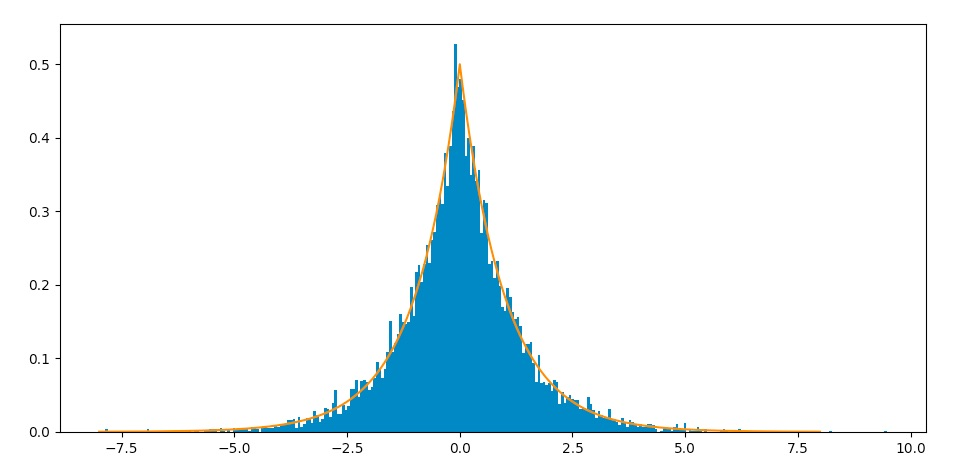
\includegraphics[scale=0.42]{images/Laplace1.jpg}
  \caption{Συνάρτηση πυκνότητας πιθανότητας κατανομής \textlatin{Laplace}, με παράμετρο κλίμακας $b=1$
}
  %\label{fig:boat1}
  \end{center}
\end{figure}


\begin{definition}(Ευαισθησία)\\
 Η $l_1$-ευαισθησία (\textlatin{sensitivity}) μιας συνάρτησης $f:X \longrightarrow \mathbb{R}^k$ είναι:
$$\Delta=max_{x\sim x'}||f(x)-f(x')||$$
\end{definition}
Η ευαισθησία μιάς επερώτησης $q$ καταγράφει το μέγεθος με το οποίο τα δεδομένα μιας και μόνο εγγραφής μπορούν να μεταβάλλουν την επερώτηση στην «χειρότερη» περίπτωση, και αντίστοιχα, τον θόρυβο που πρέπει να εισάγουμε στο αποτέλεσμα ώστε να αποκρύψουμε την συμμετοχή μιας εγγραφής στη βάση. 
Είναι προφανές ότι ένα \textlatin{counting query} έχει ευαισθησία $\Delta=1$.


\begin{theorem}(Μηχανισμός \textlatin{Laplace})\\
Έστω επερώτηση $q$ με σύνολο τιμών $\mathbb{R}$, και έστω $\Delta$ η $l_1$-ευαισθησία της. Τότε ο μηχανισμός 
$$M(x) = q(x) + z$$
με $z\sim Lap(\Delta|\epsilon)$, παρέχει $\epsilon$-διαφορική ιδιωτικότητα.
\end{theorem}

Το μέγεθος του θορύβου εξαρτάται από το είδος της επερώτησης και την επιλογή του $\epsilon$. Άρα για ένα \textlatin{counting query} θέλουμε θόρυβο τάξης $\sim Lap(1|\epsilon)$, ενώ όσο η τιμή του $\epsilon$ μικραίνει, τόσο το αποτέλεσμα γίνεται περισσότερο ανακριβές.

Θωρείστε την βάση δεδομένων $x$ με τους μισθούς που αναφέραμε προηγουμένως, και την επερώτηση για τον μέσο μισθό:
$$q(x)=\frac{\sum_{i=1}^{n}x_i}{n}$$
με $x_i\in [0,x_{max}]$. Αν χρησιμοποιήσουμε μια σχέση γειτνίασης τύπου $|x_i - x_i'|\leq x_{max}$ τότε η ευαισθησία της επερώτησης θα είναι 
$$\Delta=max_{x\sim x'}|q(x)-q(x')|=\frac{1}{n}max_{x_i,x'_i}|x_i - x'_i|\quad  i \in [1,n]$$ Έτσι έχουμε
$$\Delta=\frac{x_{max}}{n}$$
Σύμφωνα με το παραπάνω θεώρημα λοιπόν, ο μηχανισμός
$$M(x)=\frac{\sum_{i=1}^{n}x_i}{n}+Lap(\frac{x_{max}}{n\epsilon})$$
θα διατηρεί $\epsilon$-διαφορική ιδιωτικότητα.
Παρατηρούμε ότι το μέγεθος του θορύβου που προκύπτει από τον μηχανισμό \textlatin{Laplace} είναι αντιστρόφως ανάλογο του πλήθους $n$ των εγγραφών, πράγμα αναμενόμενο αφού διαισθητικά αναμένουμε καλύτερη ιδιωτικότητα αν το μέγεθος της βάσης είναι μεγάλο \textlatin{\cite{Corts2016DifferentialPI}}.

















\subsection{Εκθετικός Μηχανισμός}

Ενώ ο μηχανισμός \textlatin{Laplace} παρέχει διαφορική ιδιωτικότητα, δεν αρκεί για να καλύψει όλες τις ανάγκες, αφού εφαρμόζεται κυρίως σε επερωτήσεις που επιστρέφουν αριθμητικά αποτελέσματα. Μια χρήσιμη και αποτελεσματική μέθοδος για μη αριθμητικές επερωτήσεις είναι ο εκθετικός μηχανισμός \textlatin{\cite{dwork2008differential}}. Έδω απαιτείται η χρήση \textlatin{scoring} συναρτήσεων όπου αντιστοιχίζουν τα ζεύγη αποτελεσμάτων σε \textlatin{utility scores}. 

\begin{definition}(\textlatin{Scoring Function)}\\
Έστω $X$ το σύνολο όλων των πεπερασμένων συνόλων δεδομένων και $R$ το σύνολο τιμών ενός μηχανισμού $M$. Ως \textlatin{scoring} συνάρτηση ορίζεται:
$$u=X \times R \longrightarrow \mathbb{R}$$
και αποδίδει έναν βαθμό (\textlatin{score}) σε κάθε ζεύγος $(x,r)\in X \times R$.
 
\end{definition}
Όσο υψηλότερος είναι ο βαθμός του ζεύγους, τόσο καλύτερο το αποτέλεσμα. Η εφαρμογή που αποζητείται εδώ είναι να δίνεται μια βάση δεδομένων $x$ και ο μηχανισμός να επιστρέφει το $r\in R $ που μεγιστοποιεί τον βαθμό $u(x,r)$, ενώ παρέχει διαφορική ιδιωτικότητα.
%Παρ'όλο που η επιλογή της συνάρτησης μπορεί να γίνει αυθαιρέτως, υπάρχει συχνά φυσική επιλογή όταν η επερώτηση επιστρέφει το βέλτιστο αποτέλεσμα σε ένα πρόβλημα βελτιστοποίσης. 

Πριν παρουσιάσουμε τον εκθετικό μηχανισμό θα δώσουμε τον ορισμό της ευαισθησίας μιας \textlatin{scoring} συνάρτησης.

\begin{definition}
Η ευαισθησία μιας \textlatin{scoring} συνάρτησης $u=X \times R \longrightarrow \mathbb{R}$ είναι
\[ \Delta_u=\max_{r\in R} (\max_{x\sim x'}|u(x,r)-u(x',r)|)\]
\end{definition}

\begin{definition}(Εκθετικός Μηχανισμός)\\
Ως εκθετικός μηχανισμός ορίζεται μια τυχαιοποιημένη συνάρτηση $M_E:X\longrightarrow R$, η οποία δεδομένης βάσης $x\in X$ και παραμέτρου $\epsilon$, παράγει ένα στοιχείο $r\in R$ με πιθανότητα ανάλογη του $$ e^{\frac{e}{2\Delta_u}u(x,r)}$$
\end{definition}
Όπου $u$ είναι μια \textlatin{scoring} συνάρτηση και $\Delta_u$ η ευαισθησία της. O ορισμός συνεπάγεται το γεγονός ότι η πιθανότητα επιστροφής μιας τιμής $r$ αυξάνεται εκθετικά με την μεγιστοποίηση της τιμής $u(x,r)$. Η τιμή $r$ που μεγιστοποιεί την $u(x,r)$ έχει την μεγαλύτερη πιθανότητα.

\begin{theorem}
Ένας εκθετικός μηχανισμός παρέχει $\epsilon$-διαφορική ιδιωτικότητα.
\end{theorem}

Σε σύγκριση με τον μηχανισμό \textlatin{Laplace}, ο εκθετικός μηχανισμός είναι γενικότερος στο ότι δεν περιορίζει το ερώτημα να είναι αριθμητικό. Στην πράξη, ο εκθετικός μηχανισμός χρησιμοποιείται ευρύτερα σε περιπτώσεις όπου το σύνολο τιμών της επερώτησης είναι πεπερασμένο, έτσι ώστε η συνάρτηση πυκνότητας πιθανότητας να μπορεί να υπολογιστεί.



\subsection{Μηχανισμός \textlatin{Gauss}}

Εκτός από τον Μηχανισμό \textlatin{Laplace}, για την εφαρμογή ($\epsilon, \delta$)-διαφορικής ιδιωτικότητας σε αριθμητικές επερωτήσεις επιλέγεται και ο παρακάτω. Αρχικά δίνουμε τον ορισμό της $l2$ ευαισθησίας.

\begin{definition} 
 Η $l_2$-ευαισθησία (\textlatin{sensitivity}) μιας συνάρτησης $f:X \longrightarrow \mathbb{R}^k$ είναι:
$$\Delta_2=max_{x\sim x'}||f(x)-f(x')||_2$$
\end{definition}

Υπενθυμίζουμε την λειτουργία της ευκλείδιας νόρμας: $||x||_2=\sqrt{x_1^2+x_2^2+...+x_n^2}$

\begin{theorem}
Έστω επερώτηση $q$ με σύνολο τιμών $\mathbb{R}$ και $\Delta_2$ ευαισθησία. Για $\epsilon>0$ και $\delta>0$ ο μηχανισμός
$$M(x) = q(x) + z$$
με $z$ ένα τυχαίο διάνυσμα ανεξάρτηων τυχαίων μεταβλητών που ακολουθούν την Κανονική κατανομή με μέση τιμή 0 και διακύμανση $\sigma^2=c^2\Delta^2_2$, me $c=\sqrt{2log(1.25/\delta}/\epsilon$, παρέχει $(\epsilon, \delta)$- διαφορική ιδιωτικότητα.

\end{theorem}

 Δεν προκαλεί έκπληξη το γεγονός ότι εμφανίζεται ο όρος δ: η κατανομή \textlatin{Laplace} είναι ιδανική για πολλαπλασιαστικό φράγμα, αλλά η Κανονική κατανομή όχι.  Αν βέβαια το $\delta$ είναι επαρκώς (π.χ. λογαριθμικά) μικρό, στην πράξη δεν θα βιώσουμε ποτέ αδυναμία εγγύησης της ιδιωτικότητας. 
 
 Επίσης, ένα να απο τα πλεονεκτήματα αυτού του μηχανισμού είναι ότι το άθροισμα δυο μηχανισμών $\textlatin{Gauss}$ είναι μηχανιμός $\textlatin{Gauss}$, πράγμα που κάνει ευκολότερη την κατανόηση της εφαρμογής του κατά την ανάλυση δεδομένων. 
Οι δύο μηχανισμοί δίνουν την ίδια απώλεια αθροιστικά κατά τη σύνθεση, οπότε αν και η εγγύηση απορρήτου είναι ασθενέστερη για κάθε μεμονωμένο υπολογισμό, τα αθροιστικά αποτελέσματα μετά από πολλούς υπολογισμούς είναι ανταγωνιστικά. Τελικά προκύπτει ότι η χρήση του μηχανισμού \textlatin{Laplace} είναι καθαρότερη, ενώ οι δύο μηχανισμοί συμπεριφέρονται παρόμοια σε περιπτώσεις σύνθεσης \textlatin{\cite{Dwork:2010:BDP:1917827.1918366}}.


%Σκεφτείτε το Report Noisy Max (με τον θόρυβο Laplace) σε μια περίπτωση όπου κάθε υποψήφια παραγωγή έχει την ίδια βαθμολογία ποιότητας στη βάση δεδομένων x και στη γειτονική γ. Ανεξάρτητα από τον αριθμό των υποψηφίων αποτελεσμάτων, ο μηχανισμός αποδίδει (ε, 0) -διαπροσωπευτική ιδιωτικότητα

\section{Κατασκευή σύνθετων Μηχανισμών}

Οι μηχανισμοί που παρουσιάστηκαν παραπάνω είναι αρκετά γενικοί και απλοί στην εφαρμογή. Όπως θα δούμε και στη συνέχεια, η μόνη ποσότητα που χρειάζεται να υπολογιστεί για την υλοποίηση αυτών των αλγορίθμων είναι η ευαισθησία. Παρόλο που συνήθως υπολογίζεται εύκολα για απλές επερωτήσεις, μπορεί να είναι δύσκολο να υπολογιστεί για περίπλοκα ερωτήματα (π.χ., η βέλτιστη λύση ενός προβλήματος μη γραμμικής βελτιστοποίησης). Όταν οι επερωτήσεις είναι περίπλοκες, μια κοινή στρατηγική είναι η αποδόμηση της υπο έρευνα επερώτησης έτσι ώστε η ευαισθησία κάθε μέρους της να μπορεί εύκολα να υπολογιστεί.
Παραδείγματος χάριν, αν και η ευαισθησία της βέλτιστης λύσης ενός προβλήματος μη γραμμικής βελτιστοποίησης μπορεί να μην είναι εύκολο να υπολογιστεί, η ευαισθησία των ενδιάμεσων αποτελεσμάτων που χρησιμοποιούνται για να υπολογιστεί επαναληπτικά η βέλτιστη λύση είναι συχνά πιο απλό να υπολογιστεί. Έτσι, χρησιμοποιώντας τους κανόνες σύνθεσης, μπορεί κανείς να κατασκευάσει τον επιθυμητό μηχανισμό ιδιωτικότητας.


Τολμούμε να πούμε ότι η Διαφορική Ιδιωτικότητα αποτελεί την «ασφαλέστερη» επιλογή από τους μηχανισμούς προστασίας που αναλύσαμε. Ο κύριος λόγος είναι ότι η εφαρμογή της δεν επηρεάζεται από την γνώση που κατέχει ο επιτιθέμενος. Επιπλέον, λόγω αυτού, δεν υπάρχει και η ανάγκη μοντελοποίησης της πρότερης γνώσης, οδηγώντας σε ελαφρώς ταχύτερους αλγορίθμους. 


Στην πραγματικότητα, η Διαφορική Ιδιωτικότητα υπόσχεται να προστατεύει τα άτομα από κάθε πιθανή απειλή που θα μπορούσαν να αντιμετωπίσουν λόγω της ύπαρξης των δεδομένων τους στην ιδιωτική βάση δεδομένων $x$ και που δεν θα αντιμετόπιζαν εάν τα δεδομένα τους δεν ήταν μέρος της $x$. Παρόλο που οι εγγραφές μπορούν πράγματι να απειληθούν μόλις απελευθερωθούν τα αποτελέσματα ενός μηχανισμού ΔΙ, η διαφορική ιδιωτικότητα υπόσχεται ότι η πιθανότητα διαρροής δεν αυξάνεται σημαντικά από την επιλογή συμμετοχής τους.
Κατά κάποιο τρόπο αξιολογείται η απόφαση ενός ατόμου αν θα συμπεριλάβει ή όχι τα δεδομένα του σε μια βάση δεδομένων που θα χρησιμοποιηθεί ένας μηχανισμός ΔΙ. Εξετάζεται η διαφορά δηλαδή μεταξύ
της πιθανότητας διαρροής δεδομένου ότι συμμετέχει στη βάση, σε σύγκριση με την πιθανότητα διαρροής δεδομένου ότι δεν συμμετέχει.




 % Experiment 1

\chapter{Εφαρμογή Αλγορίθμων Διαφορικής Ιδιωτικότητας}


Στο κεφάλαιο αυτό θα περιγράψουμε τη δημιουργία προγραμμάτων ανωνυμοποίησης, χρησιμοποιώντας μηχανισμούς Διαφορικής Ιδιώτικότητας. Στη συνέχεια κάνουμε χρήση των αλγορίθμων αυτών με επερωτήσεις πάνω σε σύνολα δεδομένων. Τέλος εξάγουμε συμπεράσματα από την εφαρμογή των μηχανισμών. 

\section{Υλοποίηση}

 Η αρχιτεκτονική των μοντέλων που διαχειρίζονται τους μηχανισμούς τυχαιοποίησης είναι εντελώς διαφορετική από αυτήν των μηχανισμών γενίκευσης που αναλύσαμε. Όπως είδαμε στο κεφάλαιο 3, η τεχνική που χρησιμοποιούν οι περισσότεροι αλγορίθμοι είναι να δέχονται ένα σύνολο δεδομένων, και να επιστρέφουν μια ανωνυμοποιημένη εκδοχή του. Σε αυτή τη νέα βάση εργάζονται στη συνέχεια οι αναλυτές. Η χρήση διαδραστικών τεχνικών απαιτεί διαφορετική μοντελοποίηση: Από την μια μεριά, ο αναλυτής θέτει την επερώτησή του στην βάση δεδομένων, ενώ από την άλλη ο διαχειριστής επιλέγει το μέγεθος ιδιωτικότητας που επιθυμεί\footnote{Επιλογή της παραμέτρου $\epsilon$}. Τα δεδομένα επεξεργάζονται, προστίθεται ο θόρυβος και το αποτέλεσμα επιστρέφει στον αναλυτή.

Στο πρόγραμμα μας, θα κάνουμε χρήση κυρίως του μηχανισμού \textlatin{Laplace}, ο οποίος ικανοποιεί το κριτήριο της ΔΙ όπως δείξαμε στο προηγούμενο κεφάλαιο. 

Η συνάρτηση πυκνότητας πιθανότητας για μέσο $\mu=0$ είναι 
$$f(x|0,b)=\frac{1}{2b}e^{-\frac{|x|}{b}}$$

άρα έχουμε την αθροιστική συνάρτηση κατανομής:
$$F(x)=
\int_{-\infty}^{x} f(u)du=
\int_{-\infty}^{x} \frac{1}{2b}e^{-\frac{|u|}{b}}du=
 \begin{cases} 
      \frac{1}{2}e^{\frac{x}{b}} & x< 0 \\
      1-\frac{1}{2}e^{\frac{-x}{b}} & x\geq 0 
   \end{cases}$$
Η αντίστροφη συνάρτηση είναι:
$$F^{-1}(x)=
\begin{cases} 
      b\cdot ln(2x) & 0<x<1/2 \\
      -b\cdot ln(2-2x) & 1/2 \leq x \leq 1
   \end{cases}$$
 Θέτωντας $u=x-1/2$ καταλήγουμε σε μια γεννήτρια τυχαίων μεταβλητών:
$$X=-b\cdot sgn(u)ln(1-2|u|) \quad u\in \Big(-\frac{1}{2}, \frac{1}{2}\Big]$$

Έτσι, επιλέγοντας τυχαίες μεταβλητές $u$ από την ομοιόμορφη κατανομή στο διάστημα  $[-0.5, 0.5]$ , η τυχαία μεταβλητή $X$ θα ανήκει στην κατανομή \textlatin{Laplace} με παράμετρο κλίμακας $b$. 

Κατασκευάζουμε δυο διαφορετικές συναρτήσεις. Η μια ως είσοδο δέχεται παράμετρο $b$ και πλήθος μεταβλητών που επιθυμούμε, ενώ η δεύτερη την παράμετρο $\epsilon$ και διάσταση βάσης δεδομένων.
H σχέση που συνδέει το $\epsilon$ με την παράμετρο $b$ είναι 
$$b=\frac{\Delta f}{\epsilon}$$
με $\Delta f$ να συμβολίζει την ευαισθησία  μιας συνάρτησης $f:X \longrightarrow \mathbb{R}^k:$

$$\Delta f=max_{x\sim x'}||f(x)-f(x')||$$
όπου $x,x'$ δύο γειτνιάζουσες βάσεις δεδομένων\footnote{
Σε περίπτωση που απαιτηθεί αυστηρή εφαρμογή του ορισμού της ευασθησίας: Για την δημιουργία της βάσης $x'$, έχουμε αναπτύξει την συνάρτηση «\textlatin{falsedata}», η οποία έχει ως είσοδο την αρχική βάση $x$ και ως έξοδο μια νέα βάση η οποία διαφέρει από την αρχική το πολύ σε μια εγγραφή. Η συνάρτηση επιλέγει τυχαία μια πλειάδα της βάσης, και μεταβάλει τις τιμές των αντίστοιχων γνωρισμάτων με τυχαίο τρόπο:
\begin{itemize}
    \item Για αλφαριθμητικά γνωρίσματα, επιλέγει μια τιμή από το πεδίο τιμών του αντίστοιχου γνωρίσματος.
    \item Για αριθμητικά γνωρίσματα, η συνάρτηση εντοπίζει την ελάχιστη και την μέγιστη τιμή του γνωρίσματος και επιλέγει μια τυχαία τιμή σε αυτό το διάστημα. Έτσι διασφαλίζεται η επιπλέον διατήρηση της ιδιωτικότητας ειδικά αν αυτό το γνώρισμα είναι ευαίσθητο.
    \item Για τα λογικά γνωρίσματα (στην περίπτωση της δικής μας βάσης, οι τιμές είναι \textlatin{YES} ή \textlatin{NO}),
    επιλέγεται τυχαίως μια εκ των δύο τιμών, αλλά με πιθανότητα αντίστοιχη της εμφάνισης στη βάση. Δηλαδή αν το γνώρισμα παίρνει τις τιμές 0 ή 1, και οι άσσοι είναι 9πλάσιοι από τα μηδενικά, θα επιλεγεί η τιμή 1 με πιθανότητα 90\%. 
\end{itemize}
}.




\clearpage
Το σύνολο δεδομένων που χρησιμοποιούμε στα πειράματα είναι ένας πίνακας εκπαιδευτικών ΠΕ19 Πληροφορικής του Υπουργείου Παιδείας\footnote{\textlatin{\url{http://e-aitisi.sch.gr}}}. Αφού μετατρέψαμε τους χαρακτήρες από ελληνικά σε λατινικά, αφαιρέσαμε περιττά και ευαίσθητα γνωρίσματα. Καταλήγουμε στην τελική μορφή ενός συνόλου δεδομένων που αποτελείται από 1400 περίπου εγγραφές και έχει τα γνωρίσματα \{Όνομα, Μόρια, Παιδαγωγικό, Βαθμός, Τρίτεκνος\}. Συγκεκριμένα:
\begin{itemize}
    \item Όνομα: Το μικρό όνομα του ατόμου
    \item Μόρια: Τα μόρια που έχει συγκεντρώσει (θεωρείται ευαίσθητο χαρακτηριστικό)
   \item Παιδαγωγικό: \textlatin{YES} Αν διαθέτει παιδαγωγική πιστοποίηση, \textlatin{NO} διαφορετικά.
   \item Βαθμός: Βαθμός πτυχίου (θεωρείται ευαίσθητο χαρακτηριστικό)
   \item Τρίτεκνος: \textlatin{YES} Αν έχει τρία παιδιά τουλάχιστον, \textlatin{NO} διαφορετικά.
    
    
\end{itemize}


\begin{figure} [ht]
\begin{center}
  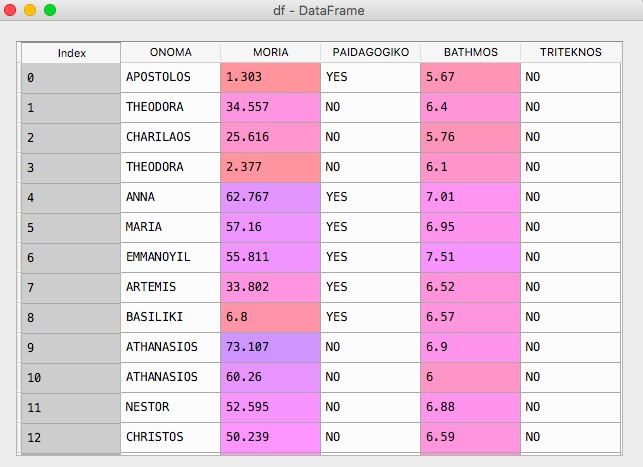
\includegraphics[scale=0.55]{images/DF.jpg}
  \caption{Πίνακας αναπληρωτών εκπαιδευτικών ΠΕ19, μετά από ανωνυμοποίηση.}
  %\label{fig:boat1}
  \end{center}
\end{figure}


Η επιλογή της βάσης έγινε λόγω των χαρακτηριστικών της, τα οποία θα μας καλύψουν στους υπολογισμούς που επιθυμούμε να πραγματοποιήσουμε. Επιπλέον, το μεγέθος είναι ιδανικό για να εμφανιστούν τυχόν σφάλματα από κακή επιλογή παραμέτρων. 






\clearpage
\section{Εφαρμογή και αξιολόγηση}

Η ανάπτυξη του αλγορίθμου γίνεται σε γλώσσα \textlatin{Python}, έκδοσης 2.7.15, σε σύστημα \textlatin{OS X} υπολογιστή \textlatin{Mac}, με διπύρινο επεξεργαστή συγχρονισμένο στα 2.4 \textlatin{GHz}. Κάνουμε χρήση των βιβλιοθηκών $Numpy$  kαι $Pandas$, ενώ η υλοποίηση γίνεται στο περιβάλλον προγραμματισμού  \textlatin{Spyder}.
 

\subsection{Δημοφιλή ονόματα}

Στο πείραμα αυτό θα εφαρμόσουμε την επερώτηση "ποιό είναι το πιο συνηθισμένο όνομα στη βάση δεδομένων?".

Υλοποιούμε μια συνάρτηση που δεχεται ως όρισμα την βάση δεδομένων, μετρά το πλήθος του κάθε ονόματος και επιστρέφει αυτό με την μέγιστη τιμή. Υλοποιούμε και μια συνάρτηση τυχαιοποίησης, που δέχεται ως όρισμα την βάση και την παράμετρο $\epsilon$ και πραγματοποιεί ακριβώς την ίδια διαδικασία, αλλά στο τέλος προσθέτει θόρυβο από την κατανομή \textlatin{Laplace}.

Η ευαισθησία της επερώτησης θα είναι $\Delta_f=1$, οπότε η παράμετρος κλίμακας της \textlatin{Laplace} είναι $b=\frac{1}{\epsilon}$.

Για $\epsilon=1$ έχουμε το αποτέλεσμα:
\begin{itemize}
    \item Χωρίς θόρυβο: '\textlatin{GEORGIOS}'
     \item Με θόρυβο: '\textlatin{GEORGIOS}'
\end{itemize}



Για $\epsilon=0.4$, μετά από λίγες εκτελέσεις προκύπτει το αποτέλεσμα:
\begin{itemize}
    \item Χωρίς θόρυβο: '\textlatin{GEORGIOS}'
     \item Με θόρυβο: '\textlatin{MARIA}'
\end{itemize}

Οπότε επαληθεύουμε την πρόταση ότι όσο μικραίνει η τιμή του $\epsilon$, τόσο η απώλεια πληροφορίας μεγιστοποιείται. 

Επεκτίνουμε την επερώτηση, αναζητώντας περισσότερα του ενός ονόματα. Η επερώτηση μας είναι τύπου Ιστογράμματος (\textlatin{histogram query}), οπότε εξακολουθεί η ευαισθησία να έιναι $\Delta_f=1$. Επιλέγουμε λοιπόν να υπολογιστούν τα 12 δημοφιλέστερα ονόματα στη βάση , επιλέγοντας $\epsilon=1$.

\begin{figure} [ht]
\begin{center}
  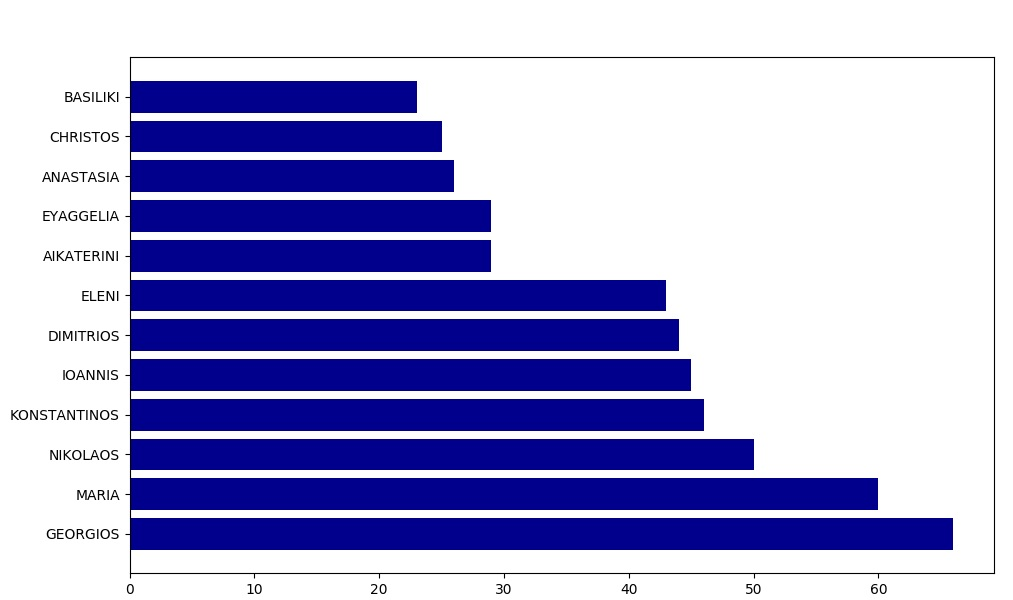
\includegraphics[scale=0.41]{images/e=1.jpg}
  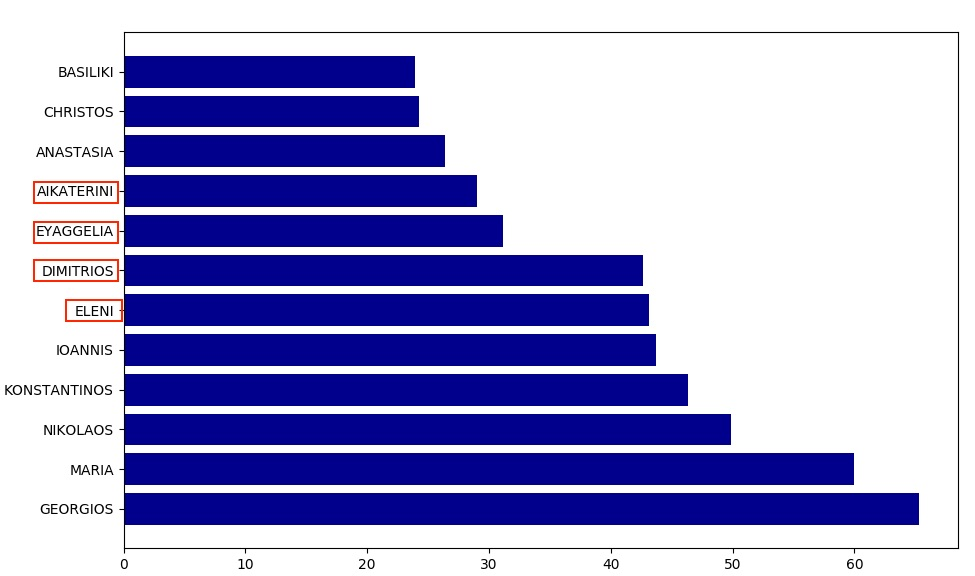
\includegraphics[scale=0.41]{images/e=2.jpg}
  \caption{Δημοφιλέστερα ονόματα - χωρίς θόρυβο (πάνω) και με θόρυβο (ε=1) (κάτω)}
  %\label{fig:boat1}
  \end{center}
\end{figure}

Παρατηρούμε ότι η πρώτη τριάδα παραμένει ανεπηρέαστη. Αντίθετα στις μεσαίες τιμές, όπου οι συχνότητες των ονομάτων είναι αρκετά κοντά, παίρνουμε εσφαλμένα αποτελέσματα. Έκτο δημοφιλέστερο όνομα στην βάση προκύπτει το '\textlatin{ELENI}', αντί του πραγματικού '\textlatin{DIMITRIOS}', παρά το ότι στην εκτέλεση της αρχικής επερώτησης η επιλογή του $\epsilon$ να έχει την τιμή 1 ήταν αποτελεσματική.

Αντιλαμβανόμαστε το μέγεθος του ζητήματος για την ορθή επιλογή της παραμέτρου $\epsilon$, το οποίο οφείλει να προβάλει τα αποτελέσματά των επερωτήσεων σε απόλυτη ισορροπία: διατηρώντας την ιδιωτικότητα των δεδομένων του συνόλου και διασφαλίζοντας την ακρίβεια του αποτελέσματος.




\subsection{Μέση τιμή}

Στο πείραμα αυτό θα εφαρμόσουμε διάφορες μορφές της κλασικής επερώτησης για την εύρεση της μέσης τιμής ενός ευαίσθητου, αριθμητικού χαρακτηριστικού.

Ξεκινάμε με την εύρεση της μέσης τιμής του γνωρίσματος '\textlatin{BATHMOS}'. Θα έχουμε λοιπόν:
$$f(x)=\frac{1}{n}\sum_{i=1}^n b_i$$

Οι τιμές των βαθμών κειμένονται στο διάστημα $[5, b_{max}]$. Παρατηρούμε ότι $$|b_i - b_i'|\leq b_{max}-5$$, συνεπώς η ευαισθησία μπορεί να υπολογιστεί ως εξής:
$$\Delta_f=max_{x\sim x'}|q(x)-q(x')|=\frac{1}{n}max_{x_i,x'_i}|b_i - b'_i|\quad  i \in [1,n]$$
Έτσι έχουμε
$$\Delta_f=\frac{b_{max}-5}{n}$$
Γνωρίζουμε ότι ο μηχανισμος
$$M(x)=\frac{\sum_{i=1}^{n}b_i}{n}+Lap(\frac{b_{max}-5}{n\epsilon})$$
θα διατηρεί $\epsilon$-διαφορική ιδιωτικότητα\textlatin{\cite{dp2}}. Εφαρμόζοντας τον τύπο στους υπολογισμούς μας παίρνουμε τα αποτελέσματα για τον μέσο βαθμό

\begin{itemize}
    \item Αρχικά: 6.74
    \item Με $\epsilon=1$: 6.74
    \item Με $\epsilon=0.1$: 6.73
    \item Με $\epsilon=0.01$: 6.81
\end{itemize}


Μια άλλη εκδοχή, είναι να προσθέσουμε θόρυβο \textlatin{Laplace} σε κάθε έναν από τους βαθμούς και να υπολογιστεί στη συνέχεια η μέση τιμή τους. Λόγω του θεωρήματος της σύνθεσης ικανοποιείται η $\epsilon$-διαφορική ιδιωτικότητα. Με αυτόν τον τρόπο μπορούμε να απεικονίσουμε και το ιστόγραμμα συχνοτήτων των βαθμών.

\begin{figure} [ht]
\begin{center}
  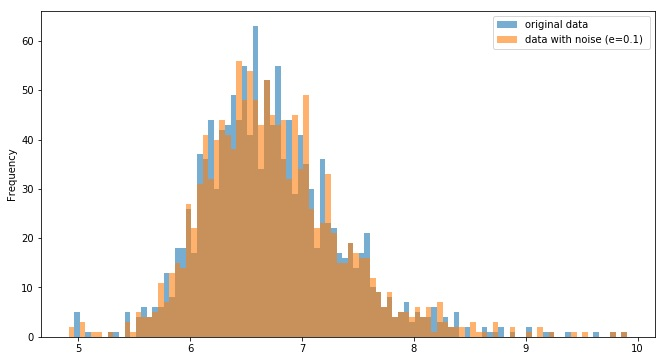
\includegraphics[scale=0.59]{images/hist01.jpg}
  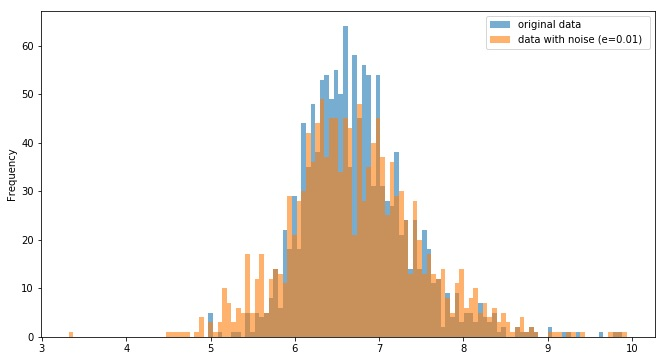
\includegraphics[scale=0.59]{images/hist001.jpg}
  \caption{Ιστόγραμμα συχνοτήτων των βαθμών}
  %\label{fig:boat1}
  \end{center}
\end{figure}

Βλέποντας τα δυο διαγράμματα συμπεραίνουμε ότι για $\epsilon=0.01$, ενώ η μέση τιμή είναι σχεδόν ανεπηρέαστη, θα υπάρχει σημαντική απόκλιση στα αποτελέσματα. Επιπλέον η διασπορά της κατανομής $Laplace$ οδηγεί στην εμφάνιση τιμών κάτω απο τη βάση του 5, πράγμα αδύνατον. 





\clearpage
\subsection{Πλήθος Τρίτεκνων}

Για τη συνέχεια των δοκιμών μας θεωρούμε το γνώρισμα "ΤΡΙΤΕΚΝΟΣ" ως ευαίσθητο, συνεπώς επερωτήσεις για συγκεκριμένες εγγραφές ως προς την τιμή του χαρακτηριστικού αυτού αποκλείονται. Μπορούμε, ωστόσο, να επερωτήσουμε συλλογικά τη βάση και να εξάγουμε συμπεράσματα. Τι γίνεται όμως στην περίπτωση που ένας επιτιθέμενος κατέχει πολύ μεγάλη γνώση για τα άτομα στην βάση?

H επερώτηση για το πλήθος των εγγραφών με θετική τιμή στο \textlatin{TRITEKNOS} επιστρέφει 32. Αυτό σημαίνει ότι η πιθανότητα ένα άτομο στη βάση να είναι θετικός στο γνώρισμα αυτό, είναι περίπου 2,3\%. Στη συνέχεια εφαρμόζουμε την επερώτηση «ποιό είναι το πλήθος των τρίτεκνων που έχουν βαθμό ίσο με 5». Η απάντηση είναι 1, ενώ το πλήθος των ατόμων με βαθμό 5 είναι τέσσερα. Η πιθανότητα επιλογής τρίτεκνου, δηλαδή, σε αυτό το υποσύνολο της βάσης είναι 25\%, δεκαπλάσια και πλέον από αυτήν επί του αρχικού συνόλου.

Υποθέτουμε τώρα ότι ο επιτιθέμενος γνωρίζει καλά τα περισσότερα άτομα στη βάση. Συγκεκριμένα ξέρει ότι ο Δημήτρης, η Φαίη και ο Ανδρέας έχουν βαθμό ίσο με 5 ακριβώς, ενώ είναι σίγουρος ότι κανείς τους δεν είναι τρίτεκνος. Σύμφωνα λοιπόν με τα παραπάνω δεδομένα, το τέταρτο άτομο του υποσυνόλου θα έχει θετική τιμή στο γνώρισμα. Προκύπτει λοιπόν αποκάλυψη του ευαίσθητου γνωρίσματος μιας εγγραφής.


\begin{figure} [h!]
\begin{center}
  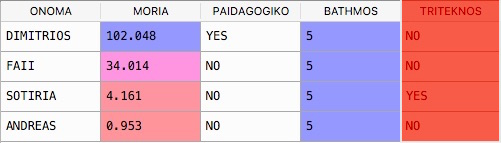
\includegraphics[scale=0.6]{images/tri1.jpg}
  \caption{Αποκάλυψη τιμής ευαίσθητου γνωρίσματος}
  %\label{fig:boat1}
  \end{center}
\end{figure}


Εφαρμόζοντας, ωστόσο, ελάχιστο θόρυβο με την μέθοδο της Διαφορικής Ιδιωτικότητας, βλέπουμε ότι η πιθανότητα αποκάλυψη της τιμής του γνωρίσματος "\textlatin{TRITEKNOS}" για μια εγγραφή είναι μηδενική.

Αν εισάγουμε θόρυβο στο γνώρισμα \textlatin{BATHMOS} όπως στην προηγούμενη παράγραφο, τότε θα είναι αδύνατο να εντοπιστούν τα 4 αυτά άτομα με βαθμό ίσο με 5. Βλέπουμε λοιπόν πως η διαφορική ιδιωτικότητα προστατεύει τα δεδομένα απο επιτιθέμενους με γνώση. 

Οι παραπάνω εφαρμογές δείχνουν ότι η εισαγωγή θορύβου στα δεδομένα και γενικά η τυχαιοποίηση είναι, θα τολμούσαμε να πούμε, η ασφαλέστερη επιλογή για την διατήρηση της ιδιωτικότητάς τους. Το μεγαλύτερο μειονέκτημα των μεθόδων αυτών είναι η επιλογή του ιδανικού μέτρου θορύβου ώστε να μην προκύψει διαστρέβλωση της πληροφορίας, ενώ ταυτόχρονα να είναι εγγυημένη η προστασία των δεδομένων. Συγκεκριμένα, στα παραπάνω παραδείγματα παρατηρήσαμε ότι η επιλογή της παραμέτρου $\epsilon$ είναι μια αρκετά επίπονη διαδικασία. Σχετικά με το θέμα αυτό έχουν γραφτεί πολλά άρθρα και έχουν προταθεί δεκάδες μέθοδοι οι οποίες αναζητούν τη «χρυσή τομή», χωρίς να προκύπτει πάντα το αναμενόμενο αποτέλεσμα από την εφαρμογή τους \textlatin{\cite{murtagh2016complexity}}.  % Experiment 2

\chapter{Συμπεράσματα - Μελλοντική Έρευνα}

Παρακάτω συνοψίζουμε τις μεθόδους που αναλύσαμε κατά τη διάρκεια της εργασίας αυτής και εξάγουμε συμπεράσματα. Στη συνέχεια αναφέρουμε επεκτάσεις, μελλοντικά έργα και νέα μοντέλα προστασίας που παρουσιάστηκαν πρόσφατα. Τέλος παρουσιάζουμε ορισμένα ανοικτά ζητήματα πάνω στην προστασία της ιδιωτικότητας των δεδομένων που θα μας απασχολήσουν στο άμεσο μέλλον.

\section{Σύνοψη και συμπεράσματα}

Στην εργασία αυτή ασχοληθήκαμε με την μελέτη των μεθόδων προστασίας της ιδιωτικότητας των δεδομένων. Μιλήσαμε για την επικινδυνότητα αποκάλυψης πληροφορίας που προκύπτει από την εφαρμογή απλών τεχνικών ανωνυμοποίησης, και την ανάγκη εισαγωγής πολυπλοκότερων μεθόδων. Αναλύσαμε τις κυριότερες τεχνικές γενίκευσης, τονίζοντας τόσο τα πλεονεκτήματα, αλλά και τα μειονεκτήματα της κάθε μιας. Παρουσιάσαμε την επίθεση τομής η οποία διαπερνά, θεωριτικά, κάθε μέθοδο γενίκευσης. Στη συνέχεια αναλύσαμε σε βάθος την μέθοδο της διαφορικής ιδιωτικότητας και τους μηχανισμούς τυχαιοποίησης που την συνοδεύουν. Τέλος, αναπτύξαμε κώδικα σε γλώσσα προγραμματισμού \textlatin{Python} που εφαρμόζει τον μηχανισμό \textlatin{Laplace} και εκτελέσαμε παραδείγματα τυχαιοποίησης σε ένα σύνολο δεδομένων.




Όπως είδαμε, ένα σύνολο δεδομένων στο οποίο έχουν εφαρμοστεί μηχανισμοί ανωνυμοποίησης μπορεί να εξακολουθεί να παρουσιάζει κινδύνους αποκάλυψης για τις εγγραφές στις οποίες αναφέρονται τα δεδομένα. Ακόμα και σε περίπτωση μη ανάκτισης της ταυτότητας ενός ατόμου, ενδέχεται να είναι εφικτή η αποκάλυψη στοιχείων σχετικά με το συγκεκριμένο άτομο με τη βοήθεια συνήθως άλλων πηγών πληροφοριών. Οφείλουμε λοιπόν να υπογραμίσουμε ότι καμία από τις τεχνικές που περιγράφονται στην παρούσα εργασία δεν πληροί με βεβαιότητα τα τρία κριτήρια της αποτελεσματικής ανωνυμοποίησης\footnote{Παράγραφος \ref{kri}}. Ωστόσο, ορισμένοι απο τους κινδύνους αυτούς ενδέχεται να μπορούν να αντιμετοπιστούν εξ' ολοκλήρου από μια συγκεκριμένη μέθοδο, δεδομένου ότι έχουν γίνει οι απαραίτητοι χειρισμοί κατα την ανάπτυξη της. Ο παρακάτω πίνακας απεικονίζει τις δυνατότητες των μηχανισμών ανωνυμοποίησης που αναλύσαμε.

\begin{figure} [h!]
\begin{center}
  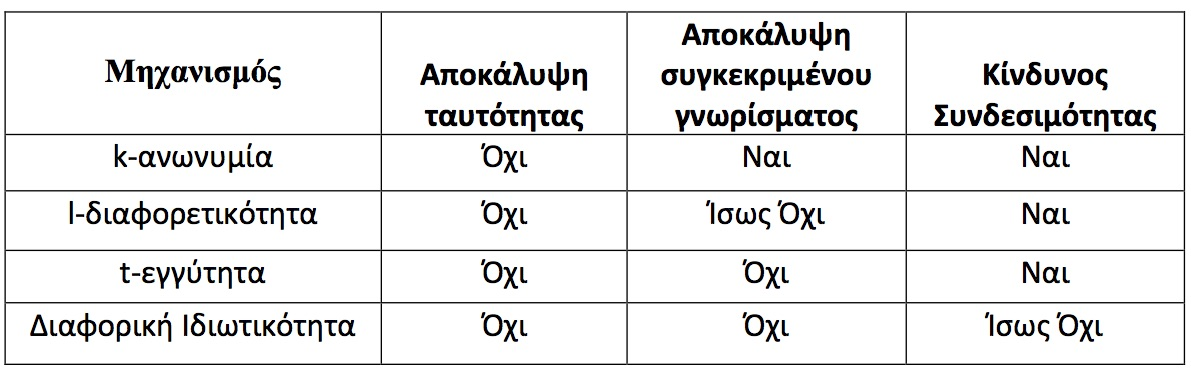
\includegraphics[scale=0.31]{images/mhx.jpg}
  \caption{Πλεονεκτήματα και μειονεκτήματα τεχνικών ανωνυμοποίησης}
  %\label{fig:boat1}
  \end{center}
\end{figure}


Συνεπώς, καλό είναι να εφαρμόζεται ο κάθε μηχανισμός ιδιωτικότητας σε αντίστοιχες περιπτώσεις ανωνυμοποίησης ανάλογα με τις απαιτήσεις του υπεύθυνου της βάσης δεδομένων ή ακόμη καλύτερα, η ταυτόχρονη χρήση διαφορετικών μηχανισμών στο ίδιο σύνολο δεδομένων. 
%Η μέθοδος της διαφορικής ιδιωτικότητας όπως είδαμε βοηθά στην επιλογή κατάλληλου επιπέδου θορύβου ώστε το αποτέλεσμα να ισορροπεί μεταξύ ποιότητας-ιδιωτικότητας. Πέραν της χρήσης του \textlatin{Laplace} και των άλλων βασικών μηχανισμών της μεθόδου, μπορεί ο διαχειριστής να χρησιμοποιήσει πιο σύνθετες εφαρμογές, ανάλογα με τις συνθήκες που αντιμετωπίζει.  






\section {Νέες τεχνικές - συνδυασμοί}

Εχουν προταθεί τον τελευταίο καιρό νέες μέθοδοι ανωνυμοποίησης δεδομένων αλλά και συνδυασμοί τεχνικών γενίκευσης-τυχαιοποίησης οι οποίες υπόσχονται ακόμη καλύτερα αποτελέσματα.

Πιο συγκεκριμένα, οι συνεχείς απαιτήσεις για προστασία των όλο και μεγαλύτερων συνόλων δεδομένων, οδηγούν σε έρευνες οι οποίες επιδιώκουν να συνδυάσουν τις μεθόδους ανωνυμοποίησης που αναφέραμε, με σκοπό ασφαλέστερα και ταχύτερα αποτελέσματα. Ένας συνδιασμός που αξίζει να ανφέρουμε είναι η χρήση τεχνικών γενίκευσης και διαφορικής ιδιωτικότητας \textlatin{\cite{DBLP:journals/corr/Domingo-FerrerS15a}}.
Στην εργασία αυτή αποδεικνύεται ότι η $k$-ανωνυμία για την προστασία των \textlatin{quasi-identifiers}, σε συνδιασμό με μηχανισμό $\epsilon$-διαφορικής ιδιωτικότητας για τα ευαίσθητα γνωρίσματα αποδίδει στοχαστική $t$-εγγύτητα \footnote{επέκταση της $t$-εγγύτητας}, με $t=t(k,\epsilon)$ συνάρτηση των $k$ και $\epsilon$. 


Πέραν αυτού, πρόσφατες έρευνες αναδεικνύουν νέα μοντέλα προστασίας της ιδιωτικότητας των δεδομένων, τόσο διαδραστικά όσο και μη διαδραστικά. 
Τελευταία, παρουσιάστηκε η τεχνική \textlatin{permutation paradigm} για να περιγράψει οποιαδήποτε μέθοδο κάλυψης δεδομένων, κυρίως \textlatin{microdata}, ως «μεταλλαγή», ανοίγοντας το δρόμο για την πραγματοποίηση ουσιαστικών αναλυτικών συγκρίσεων των μεθόδων\textlatin{\cite{domingo2016new}}. 
Η ιδιωτικότητα που εξασφαλίζεται με αυτή τη μέθοδο μπορεί να επαληθεύεται από κάθε άτομο που παρέχει τα δεδομένα του στη βάση και επίσης, στο επίπεδο συνόλου δεδομένων, από τον διαχειριστή\textlatin{\cite{ruiz2018some}}. 
Ακόμη, η τεχνική αυτή μοντελοποιεί την μέγιστη γνώση του επιτιθέμενου, ενώ προσπαθεί να προσεγγίσει την κατάσταση πλήρους διαφάνειας για τον χρήστη δεδομένων ως προς την ανωνυμοποίηση \footnote{Μόνο η τυχαιοποίηση που χρησιμοποιήθηκε πρέπει να μένει κρυφή}, δηλαδή εφαρμογή της υπόθεσης του \textlatin{Kerckhoff}\footnote{Ένα κρυπτογραφικό σύστημα πρέπει να σχεδιάζεται για να είναι ασφαλές, ακόμη και αν όλες οι λεπτομέρειες του, εκτός από το κλειδί, είναι δημοσίως γνωστές.
}.


%Πρόσφατα παρουσιάστηκαν νέοι μηχανισμοί που ικανοποιούν την διαφορική ιδωτικότητα χρησιμοποιώντας 





Η προστασία της ιδιωτικότητας των δεδομένων απαιτεί, όπως είδαμε, πολλούς πόρους και μεγάλη ακρίβεια. Είναι προφανές ότι είναι απαραίτητη η συνεχής αναζήτηση ταχύτερων αλγορίθμων ανωνυμοποίησης καθώς και ασφαλέστερων τεχνικών, οι οποίες ταυτόχρονα θα αποφέρουν μηδενική απώλεια πληροφορίας.  % Results and Discussion

%\input{Chapters/Chapter7} % Conclusion

%% ----------------------------------------------------------------
% Now begin the Appendices, including them as separate files

\addtocontents{toc}{\vspace{2em}} % Add a gap in the Contents, for aesthetics

\appendix % Cue to tell LaTeX that the following 'chapters' are Appendices

\newpage
\Huge{Παράρτημα Κώδικα}



\textlatin{\lstinputlisting[language=Python]{code/DP_names.py}}

\textlatin{\lstinputlisting[language=Python]{code/dp_algos.py}}

\textlatin{\lstinputlisting[language=Python]{code/average.py}}	% Appendix Title

%\input{Appendices/AppendixB} % Appendix Title

%\input{Appendices/AppendixC} % Appendix Title

%\addtocontents{toc}{\vspace{2em}}  % Add a gap in the Contents, for aesthetics

%\backmatter

%% ----------------------------------------------------------------


\label{Bibliography}
%\lhead{\emph{Bibliography}}  % Change the left side page header to "Bibliography"

\bibliographystyle{apalike}  % Use the "unsrtnat" BibTeX style for formatting the Bibliography
\selectlanguage{english}
\normalsize{{\bibliography{Bibliography}}}  % The references (bibliography) information are stored in the file named "Bibliography.bib"
\nocite{*}

%% ----------------------------------------------------------------

\end{document}  % The End